\documentclass[../main-v2-manifolds.tex]{subfiles}
%%%%%%%%%
%%%%%%%%%
%%%%%%%%%
\makeatletter
\newcommand*{\addFileDependency}[1]{% argument=file name and extension
\typeout{(#1)}% latexmk will find this if $recorder=0
% however, in that case, it will ignore #1 if it is a .aux or 
% .pdf file etc and it exists! If it doesn't exist, it will appear 
% in the list of dependents regardless)
%
% Write the following if you want it to appear in \listfiles 
% --- although not really necessary and latexmk doesn't use this
%
\@addtofilelist{#1}
%
% latexmk will find this message if #1 doesn't exist (yet)
\IfFileExists{#1}{}{\typeout{No file #1.}}
}\makeatother

\newcommand*{\myexternaldocument}[1]{%
\externaldocument{#1}%
\addFileDependency{#1.tex}%
\addFileDependency{#1.aux}%
}
%------------End of helper code--------------
%%%%%%%%
% PUT ALL EXTERNAL DOCUMENTS YOU WANT TO REFERENCE IN THIS SECTION
\myexternaldocument{./Preliminaries} % Reference the Preliminiaries Page
\myexternaldocument{./Symplectic-Geometry}
%%%%%%%%%
%%%%%%%%%
%%%%%%%%%
%%%%%%%%%

\begin{document}
\providecommand{\ek}{e^{2\pi k J t}}
\providecommand{\Grom}{\mathrm{Gromov}}
\providecommand{\Periodic}{\mathrm{Periodic}}
\providecommand{\frakc}{\mathcal{C}}
\providecommand{\frakco}{\mathcal{C}_0}
\providecommand{\hcal}{\mathcal{H}}
\providecommand{\hcala}{\mathcal{H}_a}
\providecommand{\osc}{\mathrm{osc}}
%%%%%%%%
%%%%%%%%
\graphicspath{{../images/}{images/}} 
%%%%%%%%
%%%%%%%%

% External Commands to be used
\fchapter{10: Equations (1)}

\topheader{Calculus}
\begin{description}
    \item[Fundamental Theorem]
    $E$ and $F$ will be Banach spaces over $\real$. Let $f:[a,b]\to E$ be a regulated mapping, the integral of $f$ with basepoint $a$ is the function 
\[
    F:[a,b]\to E,\quad F(t) = \int_a^t f(s)ds.
\]
If $f$ is continuous at $c$, then $F'(c) = f(c)$. 
\item[Derivative]
Let $U\osub E$, a mapping $f:U\to F$ is differentiable at $x\in U$ if there exists $\lambda\in L(E,F)$ where
    \[
        f(x+h) = f(x) + \lambda(h) + o(h)\qqtext{where}\lim_{h\to 0}o(h)\abs{h}^{-1} = 0.
    \]
    Derivative at $x$ is unique. If $f$ is continuously differentiable on $U$, we write $Df: U\to L(E,F)$.
    \item[Mean Value Theorems]
    Let $f\in C^1(U,F)$, and $x,y, x+y$ in some convex subset of $U$, then
    \[
        f(x+y) = f(x) +\int_0^1 \langle Df(x + ty), y\rangle dt = f(x) + \langle\int_0^1 Df(x + ty)dt, y\rangle.
    \]
    We also have the following estimates.
    \begin{align*}
        \abs{f(x+y) - f(x)} &\leq \sup\abs{Df(x+ty)}\abs{y}\\
        \abs{f(x+y) - f(x) - Df(x)(y)} &\leq \sup\abs{Df(x + ty) - Df(x)}\abs{y},
    \end{align*}
    with both supremums being taken over $0\leq t\leq 1$.
    \item[Taylor's Theorem]
    Let $f\in C^p(U,F)$, and $x,y\in U$ such that $x+ty$ is in $U$. 
    \[
        f(x+y) = f(x) + \sum_{i=\underline{p-1}}\dfrac{D^{i}f(x)(y^{(i)})}{i!} + R_p
    \]
    \item[Polynomial Estimates]
    For multi-indices $\alpha,\beta$,
    \begin{align*}
        \abs{x^\beta}&\leq (1+\abs{x})^{\abs{\beta}}\leq (1+\abs{x})^N\quad\forall \abs{\beta}\leq N\\[2ex]
        \abs{x^\alpha}&\leq (1+\abs{x}^2)^{\abs{\alpha}/2}\\[2ex]
        (1+\abs{x})^N&\Lsim_{N}\sum_{\abs{\gamma}\leq N}\abs{x^\gamma}
    \end{align*}
    \item[Weierstrass' $M$-test of Uniform Convergence]
    Let $\{f_n\}\subseteq C(X,E)$, where $E$ is a Banach space. If $\norm{f_n}_u\leq c_n$ where $c_n\in l^1$, then $\norm{\sum f_n-f}_u\to 0$ for some $f\in C(X,E)$.
    \end{description}
\topheader{Algebra}
\begin{description}
    \item[Kronecker Product]
    Let $A, B\in\real^{2\times 2}$, then
    \begin{align*}
        (A\otimes\id{\realn})(B\otimes\id{\realn}) &= AB\otimes\id{\realn}\\
        \exp(A\otimes\id{\realn}) &= \exp(A)\otimes\id{\realn}        
    \end{align*}
    \item[Symplectic Group]
    \[
    \operatorname{Sp}(n) = \bigset{M\in\real^{2n\times 2n},\ \langle Mx,\ My\rangle_{\omega_0} = \langle x,\ y\rangle_{\omega_0}}=\{M,\ M^TJM = J\}
    \]
    \item[Standard Symplectic Form]
    \[
    J_{2n} = J_2\otimes \id{\realn}\qqtext{where}J_2 = \symatrix 
    \]
    and
    \[
        \omega_0(x,y) = \langle x,\ y\rangle_{\omega_0} = \langle x,\ Jy\rangle_{\realtn}
    \]
    in coordinates
    \[
        \omega_0(x,y) = \sum_{i=\underline{n}}\det\qty(\begin{bmatrix}
            x_i & y_i \\
            x_{n+i} & y_{n+i}
        \end{bmatrix})
    \]
    \item[Exponential of $J_{2n}$]
    \[
        e^{2\pi J_2 kt}=\cos(2\pi kt)\id{\real^2} + \sin(2\pi kt)J_2,
    \]
    hence
    \[
        e^{2\pi Jkt} = \cos(2\pi kt)\id{\realtn} + \sin(2\pi kt)J_{2n}
    \]
    \item[Symplectic Pairing]
    $a: C^\infty(S^1,\realtn)\times C^\infty(S^1,\realtn)\to\real$ with 
    \[a(x,y) = 2^{-1}\int_0^1 \langle\mathring{x}(t),\ y(t)\rangle_{\omega_0}dt.\]
    \item[Symplectic Action]
    Also denoted by $a: C^\infty(S^1,\realtn)\to\real$, defined by $a(x) = a(x,x)$,
    \[
        a(x) = 2^{-1}\int_0^1\langle \mathring{x}(t),\ x(t)\rangle_{\omega_0}dt.
    \]
    \item[Symplectic Pairing is Symmetric] 
    Using integration by parts, one sees that the boundary terms vanish and the negative sign can be used to flip the arguments within the integrand (because $\omega_0$ is skew-symmetric).
    \[
        \int_0^1\langle\mathring{x}(t),\ y(t)\rangle_{\omega_0}dt = \int_0^1\langle\mathring{y}(t),\ x(t)\rangle_{\omega_0}dt.
    \]
\end{description}
\begin{remark}[$J = J_{2n}$]
        We sometimes write $J = J_{2n}$ when it is understood.
    \end{remark}
\topheader{Topology}
\begin{description}
    \item[Arzela-Ascoli's Theorem]
    Let $X$ be compact and Hausdorff, and $\{f_{\alpha}: X\to E\}$ is a family of continuous functions into a Banach space $E$ that is 1) pointwise bounded
        \[\sup_{\alpha}\norm{f_{\alpha}(x)}<+\infty\quad\forall x\in X,\]
        and 2) equicontinuous:
        \begin{quote}
        For every point $x\in X$, and $\varepsilon>0$, there exists a neighbourhood $U$ of $x$ where
        \[
            \sup_{y\in U,\alpha}\norm{f_{\alpha}(y) - f_{\alpha}(x)}\leq \varepsilon.
        \]    
        \end{quote}
        (if $E$ is infinite-dimensional, assume $\cup f_{\alpha}(X)$ is precompact as well), then $\{f_{\alpha}\}$ is totally bounded in the uniform norm, and is precompact in $C(X,E)$.
\end{description}
\topheader{Distributions}
\begin{itemize}
    \item $C_0(\realn,\realm) = \{f\in C(\realn,\realm),\  \lim_{\abs{x}\to\infty}\abs{f(x)}=0\}$, the space of continuous functions that vanish at infinity.
    \item $C^\infty(U,\realm) = \{f: U\to\realm,\  f\text{ is smoothly differentiable}.\}$.
    \item $C^\infty_c(U,\realm) = \{f\in C^\infty(\realn,\realm), \  \supp{f}\text{ is a compact subset of }U.\}$.
    \item $\szz(\realn,\realm) = \{f\in C^\infty(\realn,\realm),\  \norm{f}_{(N,\alpha)}<+\infty\: \forall N,\alpha\}$, where 
    \[
        \norm{f}_{(N,\alpha)} = \sup \abs{(1+\abs{x})^N\partial^\alpha f(x)}.
    \]
    $\szz$ is the space of Schwartz functions, or rapidly decreasing smooth functions.
    \item $C^\infty_s(\realn,\realm) = \{f\in C^\infty(\realn,\realm),\  \abs{\partial f(x)}\Lsim_{f,\alpha} (1+\abs{x})^{N(\alpha)}\ \forall\alpha\exists N(\alpha)\}$, the space of slowly increasing functions.
    \item $\szz'(\realn,\realm) = \szz(\realn,\realm)^\ast$ is the space of tempered distributions, equipped with the weak-$\ast$ topology.
    \item $c_s(\mathbb{Z},\realm) = \{f:\mathbb{Z}\to\realm,\ \abs{f(k)}\Lsim_{f}(1+\abs{k})^N\  \exists N\}$, the space of slowly increasing sequences. 
    \item $c_r(\mathbb{Z},\realm) = \{f:\mathbb{Z}\to\realm,\ \abs{f(k)}\Lsim_{N} (1+\abs{k})^{N}\ \forall N\}$, the space of rapidly decaying sequences.
\end{itemize}
\begin{definition}[Distributional Derivatives]
    Let $F\in\szz'(\realn,\real)$, for any multi-index $\alpha$, 
    \[
        \partial^\alpha F\in\szz'(\realn,\real)\qqtext{where}\langle\partial^\alpha F,\:\phi\rangle_{\szz} = (-1)^{\abs{\alpha}}\langle F,\:\partial^\alpha\phi\rangle_{\szz},\quad\forall\phi\in\szz(\realn,\real).
    \]
\end{definition}
\begin{remark}[Pointwise Multiplication]
    If $f\in \szz(\realn,\real)$, $g\in C_s^\infty(\realn,\real)$, then $fg\in \szz(\realn,\real)$; and if $f\in C_c^\infty(\realn,\real)$, $g\in C^\infty(\realn,\real)$, then $fg\in C_c^\infty(\realn,\real)$.
\end{remark}
\begin{remark}[Periodic Functions]
    We concern ourselves with periodic functions on the torus, that is: functions defined on
    \[S^1 = \{z\in\complex,\: \abs{z}=1\} \cong [0,1).\]
\end{remark}
\begin{definition}[Vector Valued Exponential]
    For $k\in\mathbb{Z}$, $E_{k}(x) = ({e^{2\pi i kx}},\ldots,{e^{2\pi i kx}})\in\complex^n$ (repeated $n$ times).
\end{definition}
\begin{definition}[Classical Fourier Transform]
    Let $1\leq p\leq 2$, the Fourier Transform of $f\in L^p(S^1,\realn)$ is 
\[
    \fourier(f):\mathbb{Z}\to\complex^n\qqtext{where}\fourier(f)(k) = \int_{S^1}f(x)E_{-k}(x)dx.
\]
The integral converges absolutely, we also write $\hat{f} = \fourier(f)$. If $q = p(p-1)^{-1}$, we have
\[
    \norm*{\hat{f}}_{l^q}\leq \norm{f}_{L^p}\qqtext{with}\norm*{\hat{f}}_{l^2} = \norm{f}_{L^2}.\footnote{It is well known that $\fourier$ is a Hilbert space isomorphism from $L^2$ into $l^2$.}
\]
\end{definition}
\begin{definition}[Distributional Fourier Transform]
    Let $F\in\szz'(S^1,\realn)$, the Fourier Transform of $F$ is 
    \[
    \hat{F}:\mathbb{Z}\to\complex^n\qqtext{where}\hat{F}(k) = \langle F,\: E_{-k}(x)\rangle_{\szz}.
    \]
\end{definition}
\begin{description}
    \item[Smooth Functions and Decay]
    The Fourier Transform converts regularity (smoothness) into decay. If $f\in C^p$, where $p\geq 1$, we have
    \[
        \langle \partial_x f,\ E_{k}\rangle_{L^2} = \int_0^1 \qty[\partial_x f(x)]E_{-k}(x)dx.
    \]
    Integration by parts yields\footnote{recall $Dm(f,g) = m(Df,g) + m(f,Dg)$ for every continuous bilinear map $m$},
    \[
        \langle \partial_x f,\ E_{k}\rangle_{L^2} = \qty\Big(f(x)E_{-k}(x))\vert_{\partial S^1} + (-1)\int_0^1 f(x)\partial_x E_{-k}(x)dx.
    \]
    The boundary terms vanish, and we are left with
    \[
        (\fourier \circ \partial_x f)(k) = (2\pi i k)\hat{f}(k)
    \]
    That is to say, 
    \[
        \norm{(2\pi i k)\hat{f}(k)}_{u}\leq \norm{\partial_x f}_{L^1}\qqtext{and}(1+\abs{k}^2)^{1/2}\abs{\hat{f}(k)}\leq C\quad\forall k\in\mathbb{Z}.
    \]
    An easy induction argument will then show
    \[
        \abs{\hat{f}(k)}\Lsim_{p} (1+\abs{k}^2)^{-p/2}
    \]
    \item[$\fourier$ maps $\szz$ into $c_s$] If $F\in\szz'$, its Fourier Transform is in $c_s(\mathbb{Z},\realn)$, that is: there exists an $N\geq 1$ such that $\abs{\hat{F}(k)}\Lsim_{F}(1+\abs{k})^N$. 
    \item[Every slowly increasing sequence is a tempered distribution] Every $g(k)\in c_s(\mathbb{Z},\realn)$ can be identified by a tempered distribution using the Fourier series
    \[
        G = \sum_{\abs{k}\leq N}E_k(x)g_k\qqtext{where}\langle G,\ \phi\rangle_{\szz}.
    \]
    The Fourier series converges in the weak-$\ast$ topology. The resulting distribution $G$ has Fourier Transform $\hat{G} = g$.
    \item[Fourier Transform of Distributional Derivatives]
    If $F\in\szz'$, and for every multi-index $\alpha$, $(\partial^\alpha F)^{\wedge} = (2\pi i k)^{\alpha}\hat{F}$.
\end{description}
\begin{remark}[Assumption of Periodicity]
    From now on, $L^2 = L^2(S^1,\realtn), \szz = \szz(S^1,\realtn)$, etc.
\end{remark}
\topheader{Topologies of Function Spaces}
\begin{description}
    \item[Smooth Functions defined on Compact K: $C^\infty(K,\real)$] $f_n\to f\in$ in $C^\infty(K)$ whenever
    \[
        \norm{\partial^\alpha f_n - \partial^\alpha f}_u \to 0\footnote{note that the supremum is taken over $K$ only, as each $f_n$ has domain $K$.}\quad\forall \alpha.
    \]
    Is a complete complete topological vector space \cite{Folland2013Real}\footnote{actually a Frechet Space}
    \item[Smooth Functions: $C^\infty(\realn,\real)$] Let $\{V_k\}$ be a precompact exhaustion of $\realn$\footnote{Each $V_k$ is open, precompact, and $V_{k}\subseteq \cl{V}_{k}\subseteq V_{k+1}$. Union covers $\realn$.}, a sequence $f_n\to f$ in $C^\infty(\realn,\realm)$ whenever
    \[
        \norm{f_n - f}_{[k,\alpha]} = \sup_{x\in \cl{V_k}}\abs{\partial^\alpha f_n(x) - \partial^\alpha f(x)}\to 0.\quad\forall k,\ \forall\alpha
    \]
    \item[Schwartz Space: $\szz(\realn,\real)$] $f_n\to f$ in $\szz$ whenever
    \[
        \norm{f_n - f}_{(N,\alpha)} = \sup_{x\in\realn}\abs{(1+\abs{x})^N\partial^{\alpha}(f_n - f)}\to 0\quad\forall\alpha\ \forall N,
    \]
    and is complete\footnote{Frechet Space}.
    \item[Test Functions: $C_c^\infty(\realn,\real)$] $f_n\to f$ in $C_c^\infty(\realn,\real)$ whenever there exists compact $K\subseteq\realn,$ such that
    \[
        \supp{f_n}\subseteq K\qqtext{and}\supp{f}\subseteq K,
    \]
    and $f_n\vert_K \to f\vert_K$ in $C^\infty(K,\real)$.\footnote{is a complete topological vector space, defined using inductive limits.}
\end{description}
\topheader{Notes \& References}
The calculus portion is taken from \cite{Lang2012Real}, which corresponds to the equations proven in Chapter XIII \S 1 to 6. For the proof of Ascoli's Theorem, see any book on real or functional analysis \cite{Folland2013Real,Lang2012Real,Yosida2012,Brezis2010Functional}. In particular, Chapter 4.6 of \cite{Folland2013Real} includes a generalization to case when $X$ is a $\sigma$-compact LCH space. We have also extended Ascoli's theorem to functions which take values in an arbitrary Banach space $E$; and one can prove this by modifying the proof in \cite{Folland2013Real}. If the range of all such $f_n$ is precompact, then its closure is totally bounded. The desired statement is then a consequence of the same $\varepsilon$-dense anchor point argument.\\

For more on distribution theory, see \cite{Folland2013Real,Yosida2012,}


\fchapter{11: Equations (2)}
\topheader{Hamiltonian Flows}
\begin{definition}[Positive Gradient Flow]\label{rmk:gradient flow}
Let $H\in C^\infty(\realtn)$, the \emph{positive gradient flow} of $H$ is the vector field $\nabla H$ such that at every point $p\in \realtn$, and $v_p\in T_p \realtn$:
\begin{quote}
    The \textbf{angle between $\nabla{H}(p)$ and $v_p$ is equal to $DH(p)(v_p)$}, where
    \begin{equation}
    H(p+v_p) = H(p) + DH(p)(v_p) + o(\abs{v_p})\quad\text{for sufficiently small }v.
    \label{eq:Frechet Derivative as best possible linear approximation}
\end{equation}
\end{quote}
By the 'angle' we refer to the Euclidean inner product which takes on values in $\real$ instead of in $[-\pi, +\pi]$. Moreover, the \emph{Euclidean gradient} of $H$ in coordinates is given by
\[\nabla H = (\partial_{\underline{2n}}H)\in\vField(\realtn).\]
\end{definition}
\begin{definition}[Hamiltonian Flow]
    The \emph{Hamiltonian flow} of $H$ is the vector field $X_H$ such that at every point $p\in \realtn$, and $v_p\in T_p\realtn$:
    \begin{quote}
        The \textbf{symplectic area from $X_H(p)$ to $v_p$ is equal to $DH(p)(v_p)$.}
    \end{quote}
    More precisely, the Hamiltonian flow of $H$ is defined by the sharpening the covector field of $H$:  $X_H = \omega_0^{\wedge}(dH)$, such that
    \begin{equation}
        \omega_0(X_H(p), v_p) = dH(p)(v_p)\quad\text{for all }p\in \realtn,\: v_p\in T_p\realtn.
        \label{eq:hamiltonian flow definition symplectic pairing}
    \end{equation}
\end{definition}
\topheader{Ellipsoids}
\begin{description}
    \item[${[r]}$ matrix for quadratic forms on $\realtn$]
    \[
    [r] = \begin{bsmallmatrix}
    r^{-2}_{\underline{n}} & 0 \\
    0 & r^{-2}_{\underline{n}}
\end{bsmallmatrix}\qqtext{such that }q(x) = \langle x, [r]x\rangle_{\realtn}\qqtext{and} \nabla q(x)  = 2[r]x.
\]
\item[Normal form] 
\[
q(x) = \sum_{i=\underline{n}}\dfrac{x_i^2 + x_{n+i}^2}{r_{i}^{2}}
\]
\[
    0< r_1\leq r_2\leq \cdots\leq r_n
\]
\item[Ellipsoid] 
    Let $q$ be a positive definite quadratic form on $\realtn$; its \emph{associated open ellipsoid}  is the subset $\Epsilon_q=[q<1]$. If $q$ is given in normal coordinates,
    \[
    \Epsilon_q = \bigset{x\in\realtn,\:\sum_{i=\underline{n}} r_j^{-2}(x_j^2 + x_{n+j}^2)<1}, \qqtext{and} \partial \Epsilon_q = \{x\in\realtn, \: q(x) = 1\}.
    \]
\item[Hamiltonian Flow] 
\[X_q(x) = \sum_{i=\underline{n}} \begin{bsmallmatrix}
    0 & \lambda_i \\
    -\lambda_i & 0
\end{bsmallmatrix}\begin{bmatrix}
    x_i \\
    x_{n+i}
\end{bmatrix}\]
\item[Eigenvalues] \[\lambda_i = 2r_i^{-2}\]
\[0<\lambda_n\leq \lambda_{n-1}\leq \cdots \leq \lambda_1\]
\item[Periods] \[\left\{(2\pi)(\lambda_i)^{-1}\right\}_{i=\underline{n}} = \left\{\pi r_i^{2}\right\}_{i=\underline{n}}\]
\[
    \text{Minimum Period} = \pi r_1^2.
\]
No critical points (except $z(t) \equiv 0$), every solution is a periodic solution.
\item[Action on the boundary of ellipsoids]
Let $q:\realtn\to\real$ is a positive definite quadratic form, then
    \[
        \pi r_1^2 = \inf\bigset{\abs{a(\gamma(t))},\: \parbox{15em}{$\gamma(t)$ is a non-degenerate closed Hamiltonian orbit on $\partial \Epsilon_q$.}},
    \]
    and the infimum is attained.
\end{description}
\topheader{Symplectic Capacities}
\begin{definition}[Symplectic capacity]
    A \emph{symplectic capacity} $\frakc$ is a function that assigns to each symplectic manifold $(M,\omega)$:  a number $\frakc(M,\omega)\in[0,+\infty]$ satisfying the following properties
    \begin{description}
        \item[Monotonicity] Given two symplectic manifolds $(M,\omega)$ and $(N,\eta)$ \textbf{of the same dimension}, if $(M,\omega)$ embeds symplectically into $(N,\eta)$, then $\frakc(M,\omega) \leq \frakc(N,\eta)$.
        \item[Conformality] If $\alpha\neq 0$ is a real number, then $\frakc(M,\alpha\omega) = \abs{\alpha}\frakc(M,\omega)$.
        \item[Non-triviality] The capacities of $B(1)$ and $Z(1)$ are equal to $\pi$, \textbf{across all $n$}.
    \end{description}
\end{definition}
\begin{wts}[Capacities of dilated subsets of $\realtn$]
    Let $U$ be an open subset of $\realtn$, then $(U,\omega_0)$ is a symplectic manifold that is symplectically embedded into $(\realtn,\omega_0)$, and $\frakc(\alpha U,\omega_0) = \abs{\alpha}^2\frakc(U,\omega_0)$ for all $\alpha\neq 0$, where $\alpha U = \{x,\: \alpha^{-1} x\in U\}$.
\end{wts}
\begin{wts}[Capacities of ellipsoids of $\realtn$]
    Let $\frakc$ be a capacity, then $\frakc(\Epsilon,\omega_0) = \pi r_1^2$ for every open ellipsoid $\Epsilon$ with $r(\Epsilon) = (r_1,\ldots, r_n)$.
\end{wts}
\begin{remark}[Capacities of bounded subsets of $\realtn$]
    By monotonicity, one sees that if $U$ is an open, precompact subset of $\realtn$, $0<\frakc(U,\omega_0)<+\infty$ for every capacity $\frakc$. However, there are compact symplectic manifolds which have infinite capacity.
\end{remark}
\subsubsection*{Special symplectic manifolds}
\begin{description}
    \item[open $r$-ball]
    \[
    B(r) = \bigset{x\in\realtn,\: \sum_{i=\underline{n}} x^2_{i} + x^2_{n+i}=\abs{x}^2<r^2}
    \]
    \item[open $r$-cylinder]
    \[
    Z(r) = \bigset{x\in\realtn,\: x^2_1 + x^2_{n+1}<r^2}
    \]
    \item[$B$ embeds into $Z$] We see that if $0<r_0\leq r_1$, $B(r_0)$ embeds symplectically into $B(r_1)$ (resp. $Z$); and it is also true that $B(r)$ is embedded in $Z(r)$
\end{description}

\topheader{Gromov's Theorems}
\begin{wts}[Gromov's Squeezing Theorem]
     Assuming the existence of a capacity $\frakc$, given positive numbers $r_0$, $r_1$, the open ball $B(r_0)$ embeds into $Z(r_1)$ symplectically if and only if $r_0\leq r_1$.
\end{wts}
\begin{definition}[Gromov's Width]
    \[
        \Grom(M,\omega) = \sup\bigset{\pi r^2,\:(B(r),\omega_0)\hookrightarrow (M,\omega) \text{ symplectically}.}.
    \]
\end{definition}
\begin{wts}[Properties of Gromov's Width]
    Gromov's width is a symplectic capacity, and it is minimal: $\Grom(M,\omega) \leq \frakc(M,\omega)$ for every symplectic manifold $(M,\omega)$ and capacity $\frakc$.
\end{wts}
% \begin{definition}[Inner capacity]
%     If $\frakc$ is a capacity, the \emph{inner capacity} of $\frakc$ is a function that assigns to every symplectic manifold $(M,\omega)$ the number
%     \[
%         \frakc^{\vee}(M,\omega) = \sup\bigset{(U,\omega),\: U\osub M\text{ and hides in } M.}.
%     \]
% \end{definition}
% \begin{definition}[Inner regularity of symplectic capacities]
%     A symplectic capacity $\frakc$ is \emph{inner regular} whenever $\frakc^\vee = \frakc$.
% \end{definition}
% \begin{wts}[Properties of the inner capacity]
%     The inner capacity is a symplectic capacity, and $\frakc^\vee\leq \frakc$ for every capacity $\frakc$.
% \end{wts}
\topheader{Orbital Capacity}
\begin{definition}[Regular Hamiltonian]
    $H\in C^\infty(M,\real)$ is in $\hcal(M,\omega)$ (regular Hamiltonians) if
    \begin{description}
        \item[Vanish on open set] Open subset $U\osub M$ where
        \[H(U) = 0=\min(H).\]
        \item[Compactly supported within manifold interior] Compact $K\subseteq M\setminus \partial M$, 
        \[H(M\setminus K) = \max(H).\]
    \end{description}
\end{definition}
\begin{definition}[$\frakco$-oscillation]
    $\osc(H) =\max(H)$ is called the \emph{$\frakc_0$-oscillation of $H$}.
\end{definition}
\begin{definition}[Admissible Hamiltonian]
    A Hamiltonian $H\in \hcal(M,\omega)$ is \emph{admissible} if all periodic orbits of $X_H$ have period $T > 1$. The space of admissible Hamiltonians on $(M,\omega)$ is denoted by $\hcala(M,\omega)$.
\end{definition}
\begin{definition}[Orbital capacity]
    The \emph{orbital capacity} of a symplectic manifold (with or without boundary) $(M,\omega)$ is denoted by $\frakc_0(M,\omega)$ and is the quantity
    \[
        \frakc_0(M,\omega) = \sup\bigset{\osc(H),\: \parbox{17em}{$H$ is an admissible Hamiltonian of $M$.}}.
    \]
\end{definition}
\topheader{Orbital Capacity Properties}
\begin{wts}[Monotonicity of $\frakco$]
    If $\varphi: M\hookrightarrow N$ is a symplectic embedding between manifolds of dimension $2n$, there exists an increasing correspondence from $\{\osc(H),\: H\in\hcal_a(M)\}$ into $\{\osc(H),\: H\in\hcal_a(N)\}$; and $\frakco(M)\leq \frakco(N)$.
\end{wts}

\begin{wts}[Conformality of $\frakco$]\label{thm:conformality of frakco}
    Let $(M,\omega)$ be a symplectic manifold. If $\alpha\neq 0$ and $F\in\hcal(M,\omega)$, we write $\wig{F}=\abs{\alpha}F$ --- which is in $\hcal(M,\omega)$, and $\osc{\wig{F}} = \abs{\alpha}\osc{F}$. If $\wig{X}_{\wig{F}}$ is the Hamiltonian flow of $\wig{F}$ under the dilated manifold $(M,\alpha\omega)$, then 
    \[
        \wig{X}_{\wig{F}} = (\sgn{\alpha})X_{F}.
    \]
    We also see that
    \begin{enumerate}
        \item $X_{F}$ and $\wig{X}_{\wig{F}}$ have identical closed (resp. closed and non-degenerate) characteristics. 
        \item The periodic orbits of $X_F$ and $\wig{X}_{\wig{F}}$ correspond to each other --- $\gamma(t)$ is a $T$-orbit of $X_F$ iff $\gamma(\sgn(\alpha)t)$ is a $T$-orbit of $\wig{X}_{\wig{F}}$; and 
        \item $X_F$ is admissible iff $\wig{X}_{\wig{F}}$ is.
    \end{enumerate}
\end{wts}
\clearpage
%% Three sketches on this page
\begin{figure}[h!]
    \centering
    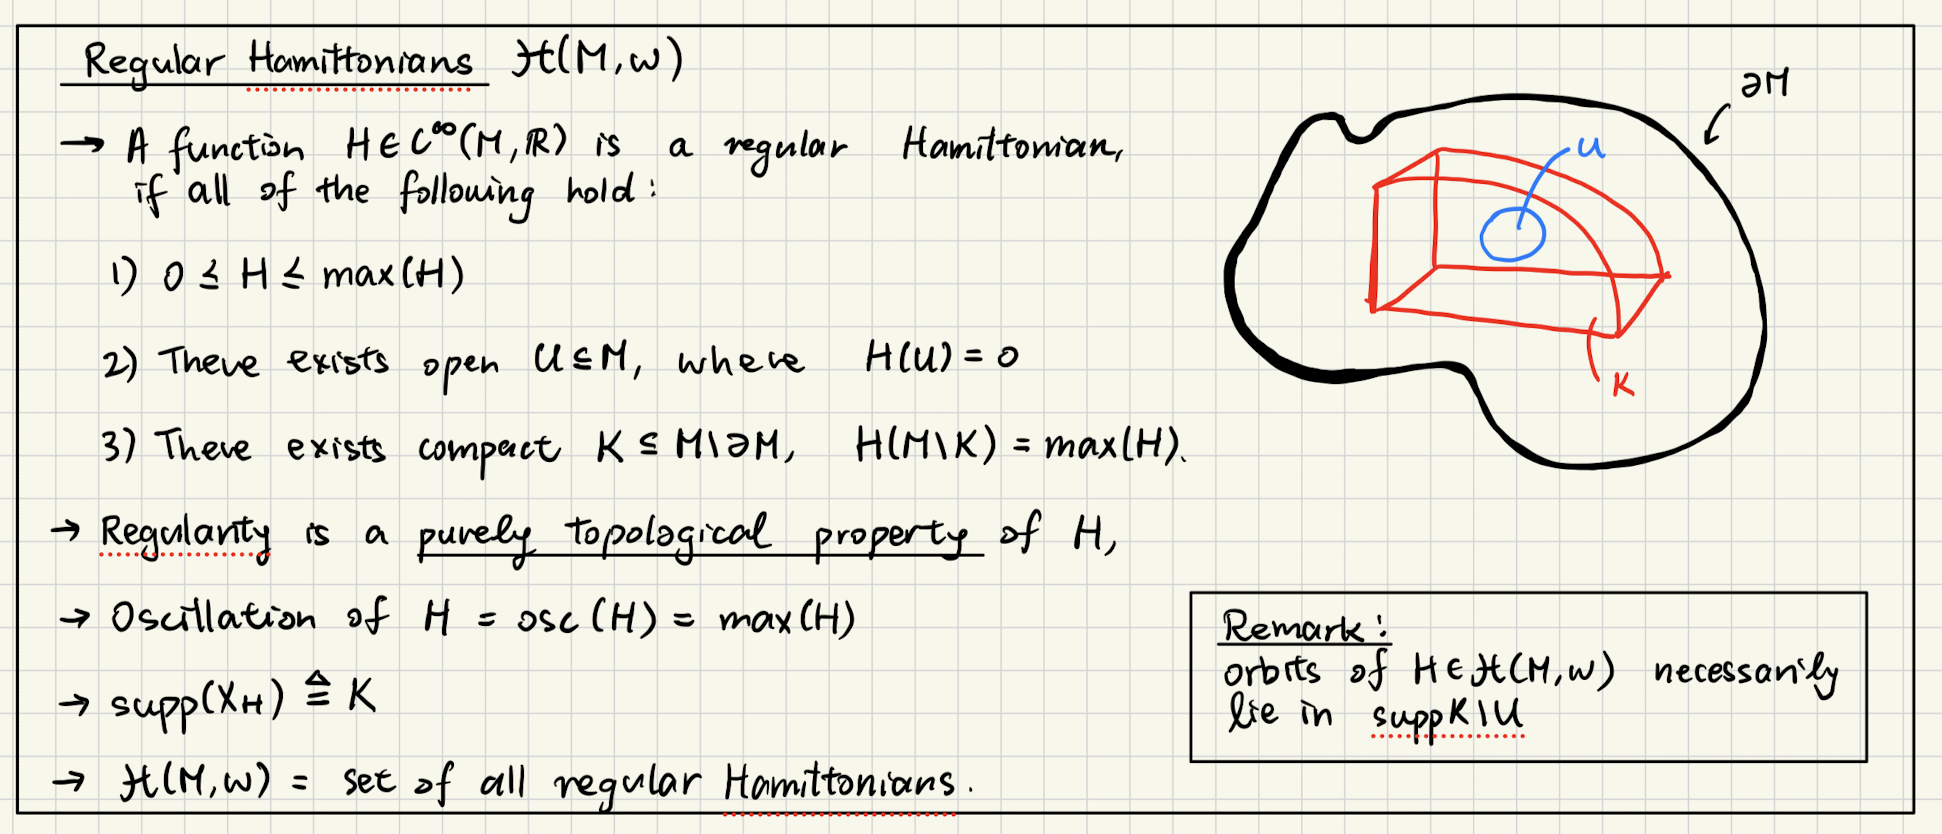
\includegraphics[width=0.85\linewidth]{images/regular-hamiltonian-sketch.png}
    \caption{Regular Hamiltonian Sketch}
    \label{fig:regular-hamiltonian-sketch}
\end{figure}
\begin{figure}[h!]
    \centering
    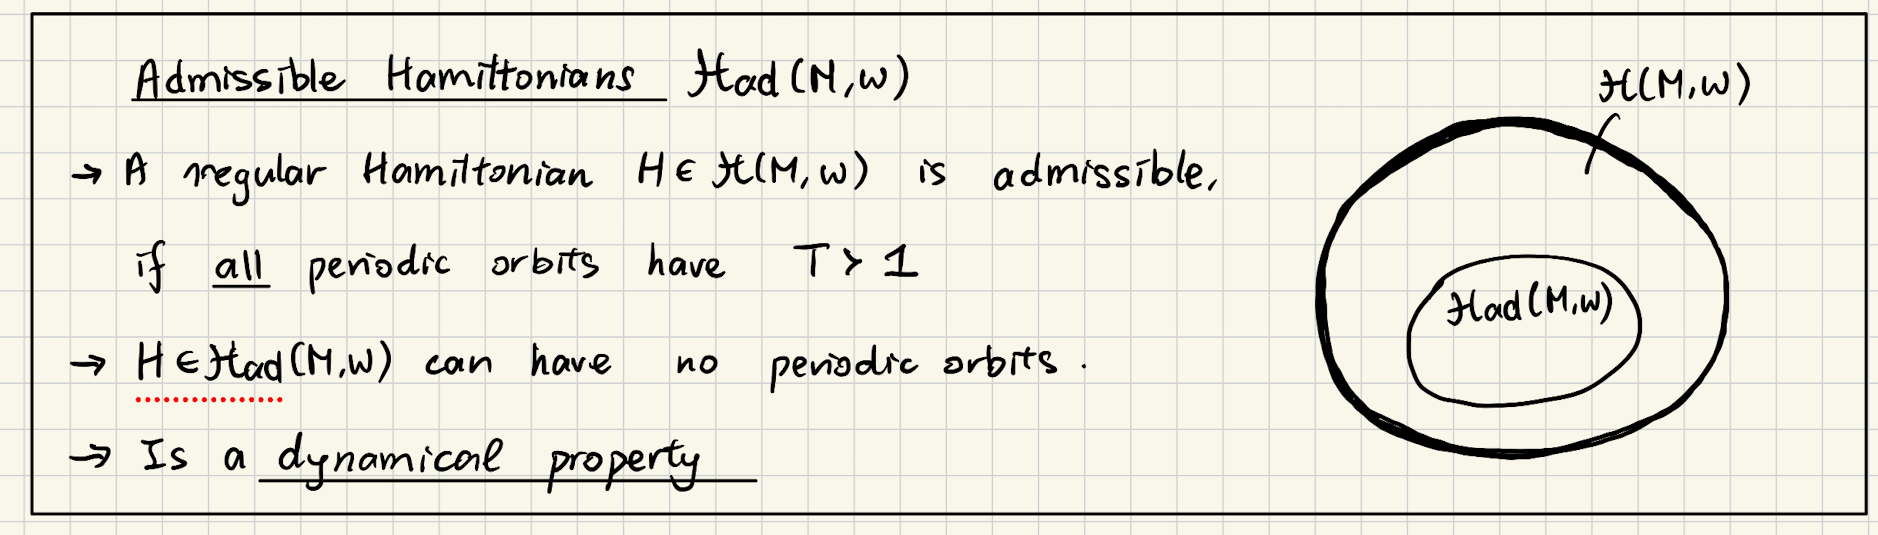
\includegraphics[width=0.85\linewidth]{images/admissible-hamiltonian-sketch.png}
    \caption{Admissible Hamiltonian Sketch}
    \label{fig:admissible-hamiltonian-sketch}
\end{figure}
\begin{figure}[h!]
    \centering
    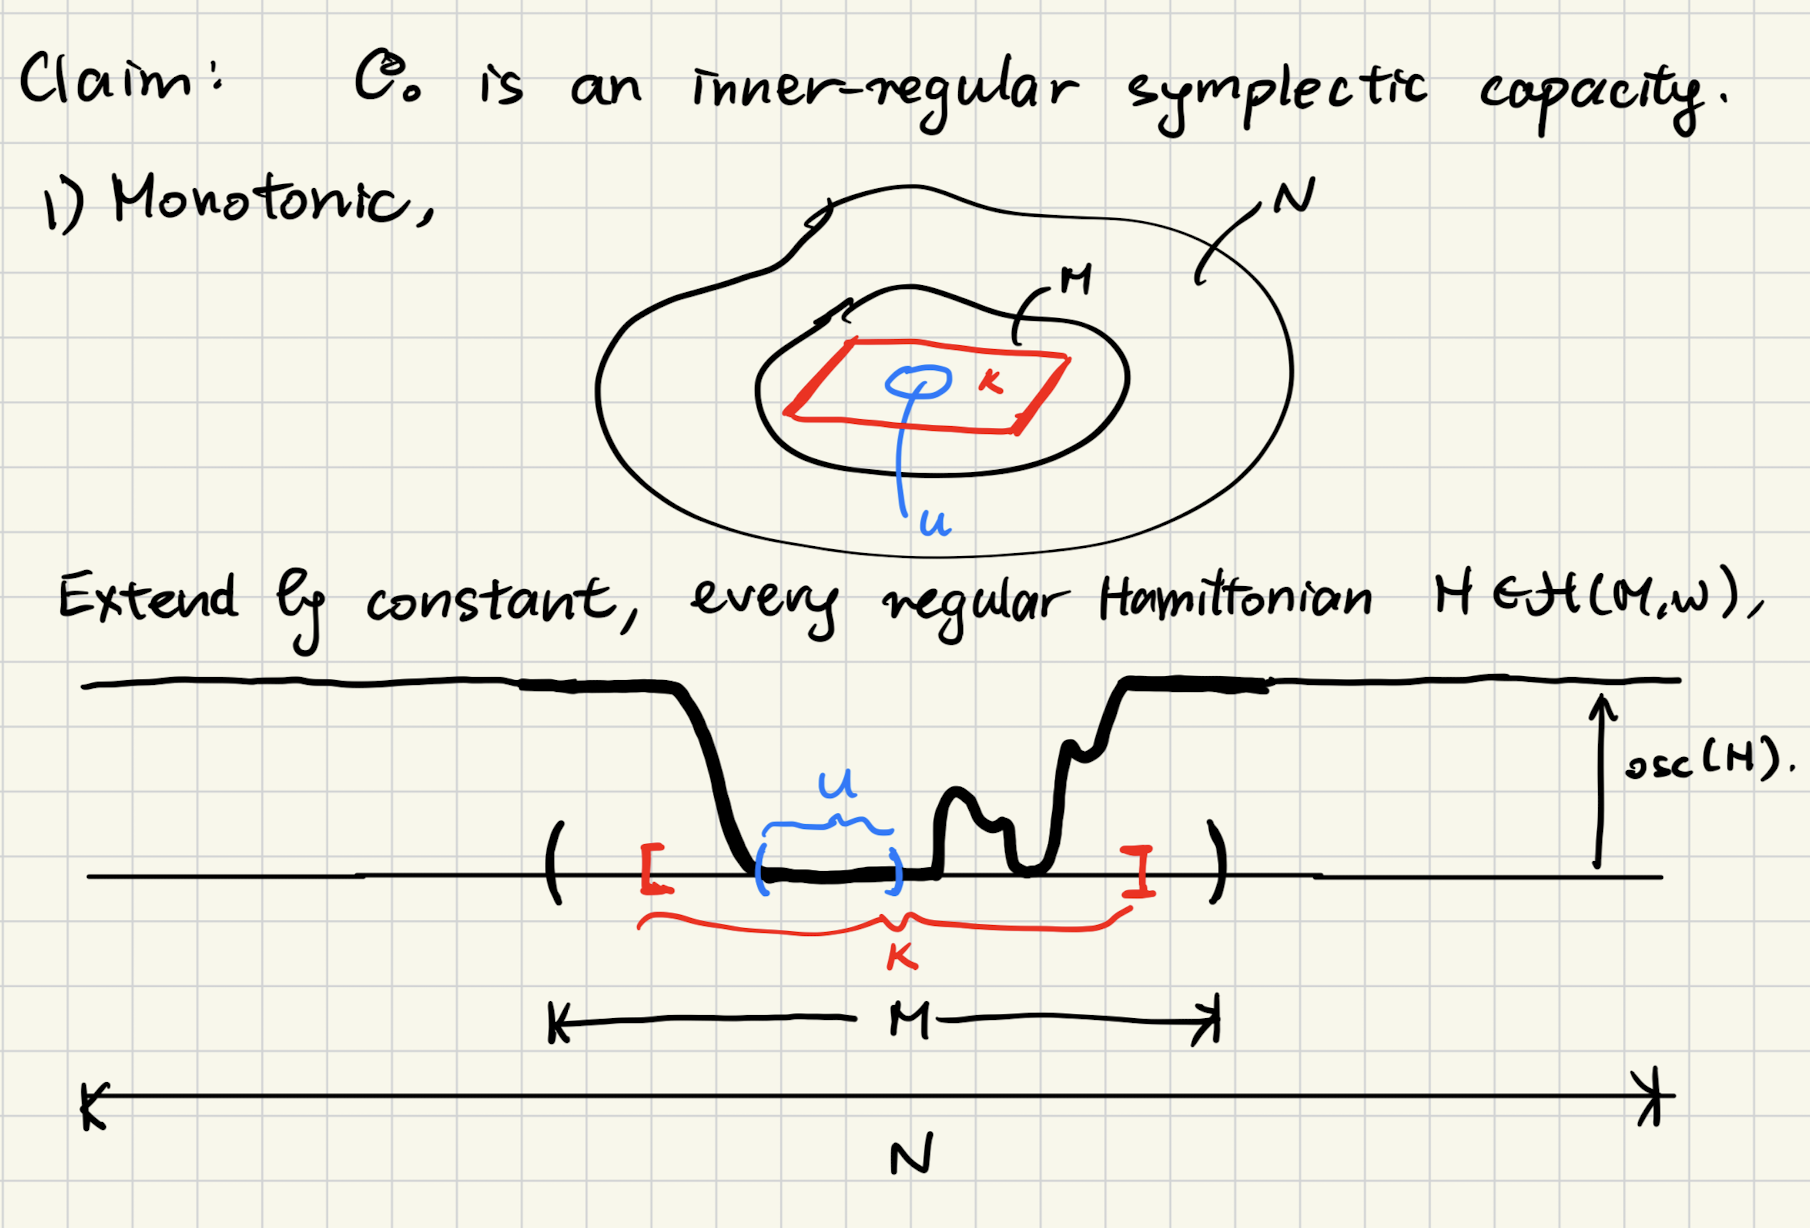
\includegraphics[width=0.85\linewidth]{images/monotonicity-orbital-capacity.png}
    \caption{Extension of a regular Hamiltonian from $M$ to $N$, is admissible iff the extension is.}
    \label{fig:monotonicity of orbital capacity sketch image}
\end{figure}
%% End of manual paeg break
\clearpage
% Poisson Bracket
\topheader{Poisson Bracket}
\begin{description}
    \item[Symplectic Manifold $(M, \omega)$] 
    $\{ F, G \}_{\text{Poisson}} = \omega(X_F,\  X_G)$
    \item[Standard Symplectic Manifold $(\realtn,\omega_0)$] $\{ F,\  G \}_{\text{Poisson}} = \omega_0 (X_F,\ X_G) = \omega_0(\nabla F,\ \nabla G)$
    \item in coordinates
    \[
    \{F,G\}_{\text{Poisson}} = \sum_{i=\underline{n}}\det\qty\Big(\begin{bmatrix}
        \partial_i f & \partial_i g \\ 
        \partial_{n+i} f & \partial_{n+i} g 
    \end{bmatrix}).
\]
\item[Lie Algebra]
\[
\mathcal{L}_{X_f}(H) = 0 \iff \mathcal{L}_{X_H}(f) = 0.
\]
\item[Conserved Quantity] $f \in C^\infty(M, \mathbb{R})$ is CQ $H$ whenever $f$ is constant on the flows of $X_H$:
\[
\mathcal{L}_{X_H}(f) = 0 \qqtext{iff} \{ f, H \}_{\text{Poisson}} = 0.
\]    
\end{description}

\topheader{Orbital Capacity Non-triviality (lower bound)}
\begin{wts}[Non-triviality of $\frakco$ (lower bound)]\label{thm:non-triviality}
We find a sequence of admissible Hamiltonians on $(B(1),\omega_0)$ with $\osc(H_n)\to \pi$, so that
\[\pi \leq c_0 (B(1), \omega_0).\]
\end{wts}
\begin{definition}[Mollifier 1]\label{def:mollifier-1}
$f \in C^\infty([0, \infty), [0, +\infty))$ with
\[
f(s) = \begin{cases}
0 \leq f'(s) < \pi &  \forall s\in[0,1] \quad \text{(Derivative Control)} \\
f(s) = 0 & \text{about } $0$ \quad \ \ \: \text{(Regularity 1)} \\ 
f(s) = \pi - \varepsilon & \text{about } $1$ \quad\ \ \:  \text{(Regularity 2)}
\end{cases}
\]
We do not specify what values $f$ will take outside of $[0,1]$.
\end{definition}


\begin{description}
    \item[Application of Derivative Control]
    Let $H\in C^\infty(\realtn,\real)$ and $f\in C^\infty(\real,\real)$, then 
    \[
        X_{f(H)}(x) = \mathring{f}(H(x))X_H(x)
    \]
    Let $\wig{T}$ be the period of any orbit $\wig{\gamma}$ of $X_{f(H)}$,
    \[
        \wig{\gamma}(t) = \underbracket{\mathring{f}\qty\Big(H\circ \wig{\gamma})}_{\text{constant}} X_H(\wig{\gamma}(t)),
    \]
    Bounding $\mathring{f}$ = bounding the periods of orbits of $f(H)$.
    \begin{align*}
    \inf\abs{\mathring{f}} &\leq \abs{\mathring{f}} \leq \sup\abs{\mathring{f}}\\
    (\sup\abs{\mathring{f}})^{-1} &\leq (\abs{\mathring{f}})^{-1} \leq (\inf\abs{\mathring{f}})^{-1}
    \end{align*}
    so that: \footnote{the inequalities below are dependent on whether or not $\sup$ or $\inf$ are attained.} 
    \[
        \dfrac{T}{\sup\abs{\mathring{f}}} \leq \wig{T} \leq \dfrac{T}{\inf\abs{\mathring{f}}}
    \]
\end{description}
\begin{definition}[Construction of admissible $H$]
    Let $H: (B(1),\omega_0)\to\real$, with $H(x) = f(\abs{x}^2)$. See \Cref{fig:mollifier-1-neck-hamiltonian}.
\end{definition}

\begin{description}
\item[Composition with Quadratic Forms]
    In general, if $q$ is a quadratic form with periods $\{\pi r_i^2\}_1^n$ and $H(x) = f(q(x))$, by the chain rule
\begin{align*}
    \nabla H(x) &= \mathring{f}(q(x))\nabla q(x) \\ 
    X_H(x) &= \mathring{f}(q(x))X_q(x)
\end{align*}
\item[Proof of \Cref{thm:non-triviality}]
In the case of $H$, we have 
\[
    \wig{T} = \dfrac{T}{\abs{\mathring{f}(\wig{\gamma})}} > \dfrac{\pi r_1^2}{\sup\abs{\mathring{f}}} > 1,
\]
Because $\osc(H) = \pi - \epsilon$, we are done. This proves
\[
\pi \leq \frakco(B(1), \omega_0) \leq \frakco(Z(1), \omega_0).
\]
\end{description}
\topheader{Construction of Mollifier 1 in \Cref{def:mollifier-1}}
It is fruitful to present a general construction of Mollifier 1.
\begin{wts}[Generalized Mollifier 1]\label{wts:generalized mollifier 1}
    Let $y_{max}>0$ and $y_0 = y_{max} - \varepsilon< y_{max}$. There exists a smooth function $f\in C^\infty([0,+\infty), \real)$ such that 
    \[
    \begin{cases}        
        0 \leq f'(s) \leq \pi-\varepsilon/2 < \pi &  \forall s\in[0,1] \quad \text{(Derivative Control)} \\
        f(s) = 0 & \text{about } $0$ \quad \ \ \: \text{(Regularity 1)} \\ 
        f(s) = y_0 & \text{about } $1$ \quad\ \ \:  \text{(Regularity 2)}
    \end{cases}    \]
\end{wts}
\begin{description}
    \item[Standard bump function] Let $\phi_0\in C_c^\infty(\real,\real)$,
        \[
        \phi_0(x) = \begin{cases}
            \exp(1/(x^2-1)) & \abs{x} < 1 \\
            0 & \abs{x}\geq 1
        \end{cases}
    \]
    We normalize $\phi(x) = (\int\phi_0(s)ds)^{-1}\phi_0(x)$. 
    \item[Shrinking the bump function]
    If $\delta>0$ we denote the $\delta$-shrinkage of $\phi$ by $\phi_{\delta}(x) = \delta^{-1}\phi(t\delta^{-1})$, so that $\int \phi_{\delta}(s)ds = 1$. Since $\supp{\phi}=[-1,\ +1]$, it follows that $\supp{\phi_{\delta}} = [-\delta,\ +\delta]$. 
    \item[Piecewise Straight Line]
    Let $l(x)$ be the unmollified version of what we want $f$ to look like. We want $l(x)$ resemble a line segment on the interval $[\frac{2}{3}\varepsilon_1,\ 1-\frac{2}{3}\varepsilon_1]$  (which has length $1-\varepsilon_1$) for some $\varepsilon_1>0$, naturally its slope should be
    \[
        \cl{m} = \dfrac{y_{max} - \varepsilon}{1-4\delta}\leq y_{max} - \varepsilon/2<y_{max}.
    \]
    By continuity, there exists such a $\delta>0$, by picking $4\delta = \varepsilon2^{-1}\min(1,y_{max}^{-1})$, and hence:
    \[
        l(x) = \min\qty\Big(y_{\max} - \varepsilon,\  \max\qty\Big(0,\ \cl{m}[x-2\delta])).
    \]
    \item[Regularity of the Convolution?]
    Here, it is useful to assume that $l(x)$ 'decreases' back down for large enough $M$. (Elaborate)?
    \item[Convolution]
    The integral defining the convolution $f(x) = (\phi_\delta\ast l)(x)$ for $x\geq 0$, and because $\phi_\delta\in L^1(x)$ and $l(x)\in L^\infty(x)$,
    \[
        f(x) = \int_{-\infty}^{+\infty}\phi_{\delta}(x-s)l(s)ds
    \]
    converges absolutely at every $x$ \cite[Thms.~~8.7, 8.10]{Folland2013Real}.
    \item[Verification of first property]
    Since $l(x)$ is globally Lipschitz, with constant
    \[
    \norm{\tau_{-z}l - l}_u=\sup_{y\in\real}\abs{l(y+z) - l(y)}\leq \cl{m}\abs{z},
    \]
    Fix any sequence $h_n\to 0$, and for all $x\geq 0$, 
    \begin{align*}
        \dfrac{f(x+h_n) - f(x)}{h_n} &= \int_{-\infty}^{+\infty}\phi_\delta(s)\qty\big[\dfrac{\tau_{-h_n}l(x-s) - l(x-s)}{h_n}]ds\\
        \abs{\dfrac{f(x+h_n) - f(x)}{h_n}}&\leq\norm{\phi_\delta}_{1}\cl{m} = \cl{m}
    \end{align*}
    \item[Verification of second and third properties]
    If $x\in [0,\ \delta]$,  the support of $\phi_\delta(x-s)$ as a function of $s$ is $[-\delta + x,\ x + \delta]$; and 
    \[
        \supp{\phi_{\delta}(x-s)}\subseteq[-\delta,\ 2\delta].
    \]
    And if $x\in [1-\delta,\ 1]$, 
    \[
        \supp{\phi_\delta(x-s)}\subseteq [1-2\delta,\ 1+\delta].
    \]
    Rewriting our piecewise line function $l(x)$, we see that 
    \[
        l(x) = \begin{cases}
            0 &  x\in[0,\ \delta] \\
            \cl{m}(x-2\delta) &  x\in[2\delta,\ 1-2\delta]\\
            y_0 &  x\in[1-\delta,\ 1]
        \end{cases}.
    \]
    The convolution integral becomes
    \[
        f(x) = \begin{cases}
            \int \phi_{\delta}(x-s)(0)ds = 0 & x\in[0,\ \delta]\\
            \int \phi_{\delta}(x-s)(y_0) = y_0 & x\in[1-\delta,\ 1].
        \end{cases}
    \]
    \end{description}
    \begin{figure}[h!]
    \centering
    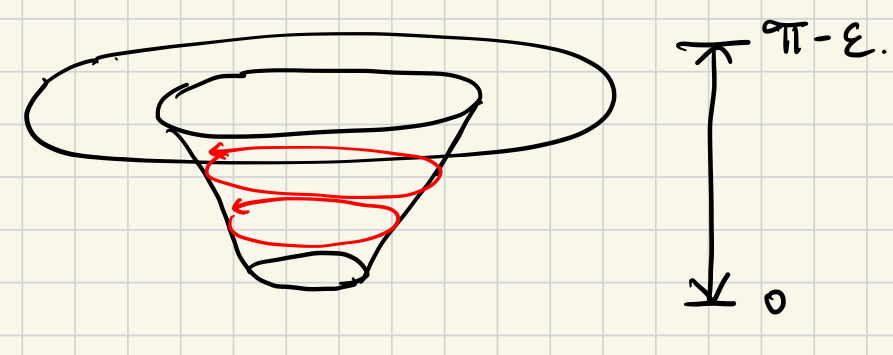
\includegraphics[width=0.75\linewidth]{images/mollifier-1-neck-hamiltonian.png}
    \caption{Admissible $H$}
    \label{fig:mollifier-1-neck-hamiltonian}
\end{figure}
\begin{figure}[h!]
    \centering
    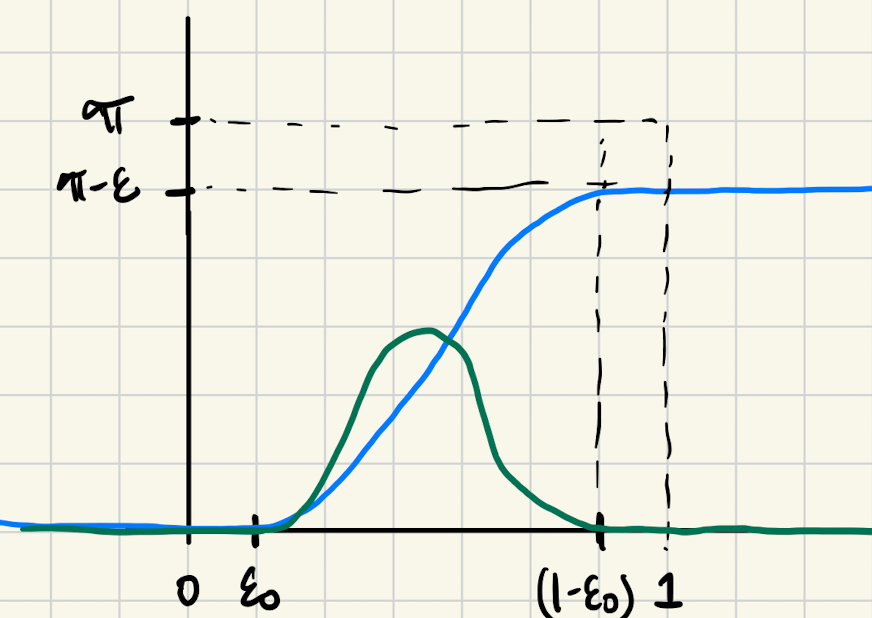
\includegraphics[width=0.7\linewidth]{images/mollifier-1-f.png}
    \caption{Mollifier 1}
    \label{fig:mollifier-1-f}
\end{figure}
\clearpage
    \topheader{General Notes for Mollifier 1}
    \begin{description}
    \item[Transition Parameters]
    Let $y_{max} = \pi$, we want to construct a mollifier $f:[0,1]\to\real$ that goes from $0$ to $y_{max} - \varepsilon$ on $[0,1]$, subject to the requirement that $f(x) = 0$ on $[0,\varepsilon_1/3]$ and $f(x) = y_{max} - \varepsilon$ on $[1-2\varepsilon_1/3]$.\\
    
    Let $\varepsilon_1 = \min(\varepsilon,\varepsilon/y_{max})/2$, we see that the number $\cl{m} = \frac{y_0}{1-\varepsilon_1}<y_{max}$. this will be the upper bound of the slope of $f$.
    \item[Transitions]
    Let $l(x)$ be the 'unmollified' version of what we want $f$ to look like.
    \[
        l(x) = \begin{cases}
            0 & x\leq 2\varepsilon_1/3\\ 
            \cl{m}(x-2\varepsilon_1/3) & 1-2\varepsilon_1/3\leq x\leq 1-2\varepsilon_1/3\\
            \pi-\varepsilon & 1-2\varepsilon_1/3\leq x
        \end{cases} = \min(1-\varepsilon,\max(0,\cl{m}(x-2\varepsilon_1/3)))
    \]
    We can smoothen $l(x)$ by convolving with the shrinked bump function using $\delta = \varepsilon_1/3$. 
    \item[Convolution]
    If $g(x) = (\phi_{\delta}\ast l)(x)$, the derivative of $g$ can be computed, 
    \[
        Dg(x) = [\phi_\delta\ast( Dl)](x)
    \]
\end{description}

\clearpage
\fchapter{12: Equations (3)}
\topheader{Introduction}
\begin{quote}
    We want to show for every $\varepsilon>0$, and for every $H\in\hcal(Z(1),\omega_0)$ with $\osc(H) = \pi + \varepsilon$, then $H$ is not admissible. 
\end{quote}
We accomplish this by finding a non-degenerate periodic orbit with $T\in (0,1]$. We make a few more reductions.
\begin{description}
    \item[Assumptions] Let $H$ be a regular Hamiltonian of $(Z(1),\omega_0)$ with 
    \[
        \pi < \pi + \varepsilon < \osc{H}
    \]
    \item[Vanish at the origin] By constructing a compactly supported symplectic diffeomorphism, we can deform the manifold such that $H\in C^\infty(Z(1),\real)$ vanishes on a neighbourhood of the origin, without destroying the orbits.
    \item[Quadratic Extension] We can extend $H$ to be a smooth function on $\realtn$ which defines a HVF. Denote this extension by $\cl{H}\in C^\infty(\realtn,\real)$.
    \item[Localization] There exists a functional $\Phi: C^\infty(S^1,\realtn)\to\real$ where
    \[
        \Phi(x) = 2^{-1}\int_0^1 \langle\mathring{x},x\rangle_{\omega_0}dt - \int_0^1 H(x)dt,
    \]
    and if $x\in C^\infty$ satisfies
    \[
        \mathring{x} = X_H(x)\qqtext{and}\Phi(x)>0,
    \]
    then $x(t)$ is a non-constant periodic orbit of the original system, meaning $x(t)\subseteq Z(1)$.
\end{description}
\topheader{Locally Hamiltonian Vector fields}
\begin{quote}
    Introduction to Smooth Manifolds - Chapter 22
\end{quote}
\begin{definition}[Locally Hamiltonian]
    $X\in \mathfrak{X}(M)$ is said to be locally Hamiltonian, if every point in $M$ admits a neighbourhood $U$ about whith $X\vert_U$ is induced by a Hamiltonian $f\in C^\infty(U,\real)$.
\end{definition}
\begin{definition}[Symplectic Vector Fields]
    $X\in\mathfrak{X}(M)$ is symplectic whenever $\omega$ is invariant under the flow of $X$.
\end{definition}
\begin{wts}[Liouville's Theorem (Hamiltonian Flows)]
    A vector field $X\in\mathfrak{X}(M)$ is locally Hamiltonian iff it is symplectic.
\end{wts}
\topheader{Straight Line Deformation}
\begin{quote}
    HZ Chapter 3.1
\end{quote}
\begin{wts}[Fattening of Compact Sets]
    Let $K$ be a compact set contained in an open neighbourhood $U$ in a locally compact metric space. There exists $\varepsilon>0$ such that the fattening
    \[
        B_{\varepsilon}(K) = \bigcup_{x\in K}B_{\varepsilon}(x)\subseteq U.
    \]
\end{wts}
\begin{wts}[Smooth Urysohn Lemma]
    Let $K$ and $U$ be as above, with the added assumption that we are in $\realn$, then there exists a smooth function $\phi\in C_c^\infty(\realn)$, where $\rho = 1$ on $\cl{B_{\varepsilon}(K)}$ and $\supp{\rho}\subseteq U$.
\end{wts}
\begin{description}
    \item We outline the construction of the deformation
    \item[Line Segment from origin] Let $z_0\in U$, and $L = \{tz_0,\ 0\leq t\leq 1\}$.
    \item[Fattening of Line Segment] Because $Z(1)$ is an open set containing $L$, we find
    \[
        L\subseteq B_{\varepsilon}(L)\subseteq \cl{B_{\varepsilon}(L)}\subseteq Z(1)
    \]
    \item[Applying Urysohn's Lemma] By $C_c^\infty$ Urysohn's Lemma, we find a smooth function $\rho$ where 
    \[
        \rho(\cl{B_{\varepsilon2^{-1}}(L)}) = 1\qqtext{and}\supp{\rho}\subseteq B_{\varepsilon}(L)
    \]
    \item[Straight Line Hamiltonian] Let $R(z) = (-1)\rho(z)\langle z, z_0\rangle_{\omega_0}$, where 
    \[X_R(z) = z_0\qqtext{whenever}z\in \cl{B_{\varepsilon2/3}(L)}.\]
    \item[Time-one map] Let $\theta = \theta^1$ be the time-$1$ map of the flow of $X_R$, it is clear that $\theta(0) = z_0$, and it maps a neighbourhood of the origin into $U\osub Z(1)$.
    \item[Regularity of $\cl{H} = H\circ\theta$ (1)] $\partial Z(1)=\varnothing$ so $\cl{H}(\theta^{-1}(U)) = 0$ for some open set, whose closure hides in the manifold interior of $Z(1)$. 
    \item[Regularity of $\cl{H} = H\circ\theta$ (2)] There exists compact $K_1\subseteq Z(1)$ such that
    \[
        \cl{H}(Z(1)\setminus K_1) = \osc(H)\qqtext{where}K_1 = \cl{\theta^{-1}(K)\cup \supp{\rho}}\quad\text{is compact}.
    \]
    \item[Conclusion] Therefore we can assume $H$ vanishes in some neighbourhood of the origin.
\end{description}

\begin{figure}[h!]
    \centering
    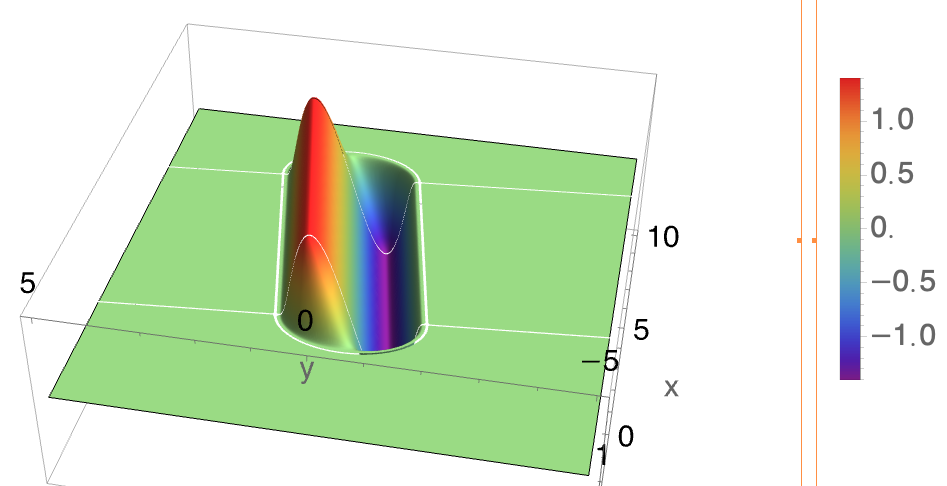
\includegraphics[width=1.1\linewidth]{images/straight-line-deformation.png}
    \caption{Straight Line Deformation 1, \texttt{straight-line-deformation.nb}}
    \label{fig:straight-line-deform 1}
\end{figure}

\begin{figure}[h!]
    \centering
    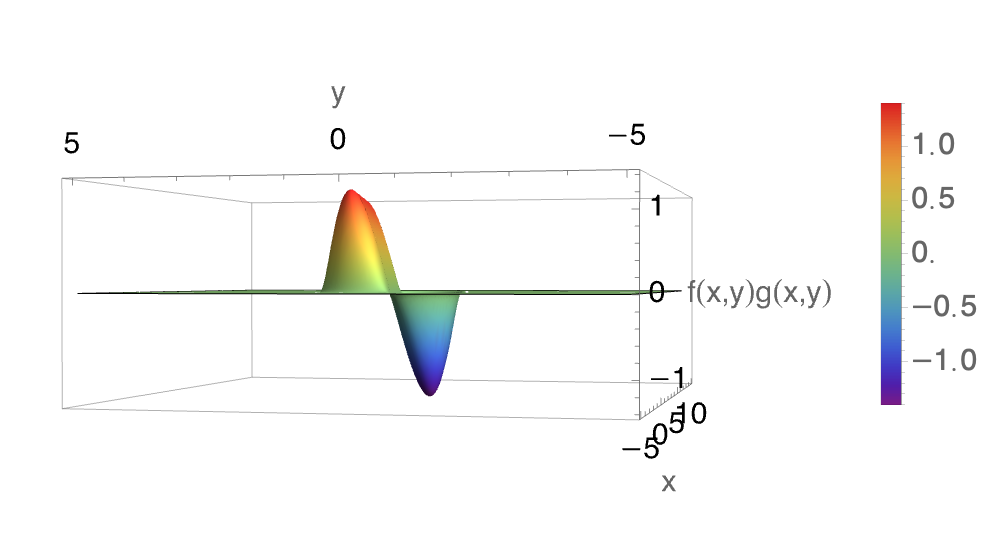
\includegraphics[width=1.1\linewidth]{images/straight-line-deformation-2.png}
    \caption{Straight Line Deformation 2}
    \label{fig:straight-line-deform 2}
\end{figure}
\clearpage
\topheader{Engulfing Ellipsoid}
\begin{description}
    \item[Special Quadratic Form]
    Because $K = \supp{H}$ is compact, there exists a large $N$ such that 
\[
    q(x) = x_1^2 + x_{n+1}^2 + N^{-2}\sum_{i\neq 0}x_i^2 + x_{n+i}^2,
\]
means $K\subseteq \{q<1\} = E$. See \Cref{fig:engulfing-ellipsoid}.
\item[Eigenvalues] 
\[
    \lambda_i = 2r_i^{-2} \qqtext{or}\{\lambda_i\} = \{2,2N^{-2}\}.
\]
\item[Periods] 
\[\{\pi,\pi N^2\}\]
\end{description}
% \begin{figure}[h!]
%     \centering
%     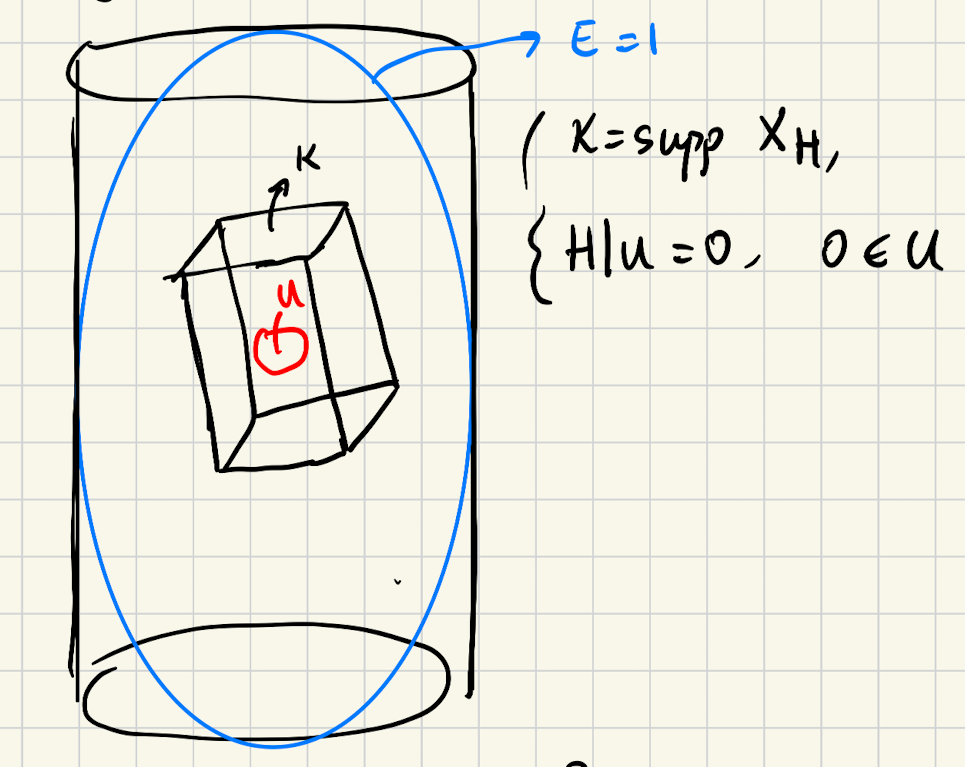
\includegraphics[width=0.5\linewidth]{images/cylindrical-ellipsoid.png}
%     \caption{Ellipsoid $q$ for large $N$}
%     \label{fig:engulfing-ellipsoid}
% \end{figure}
\begin{figure}[h!]
    \centering
    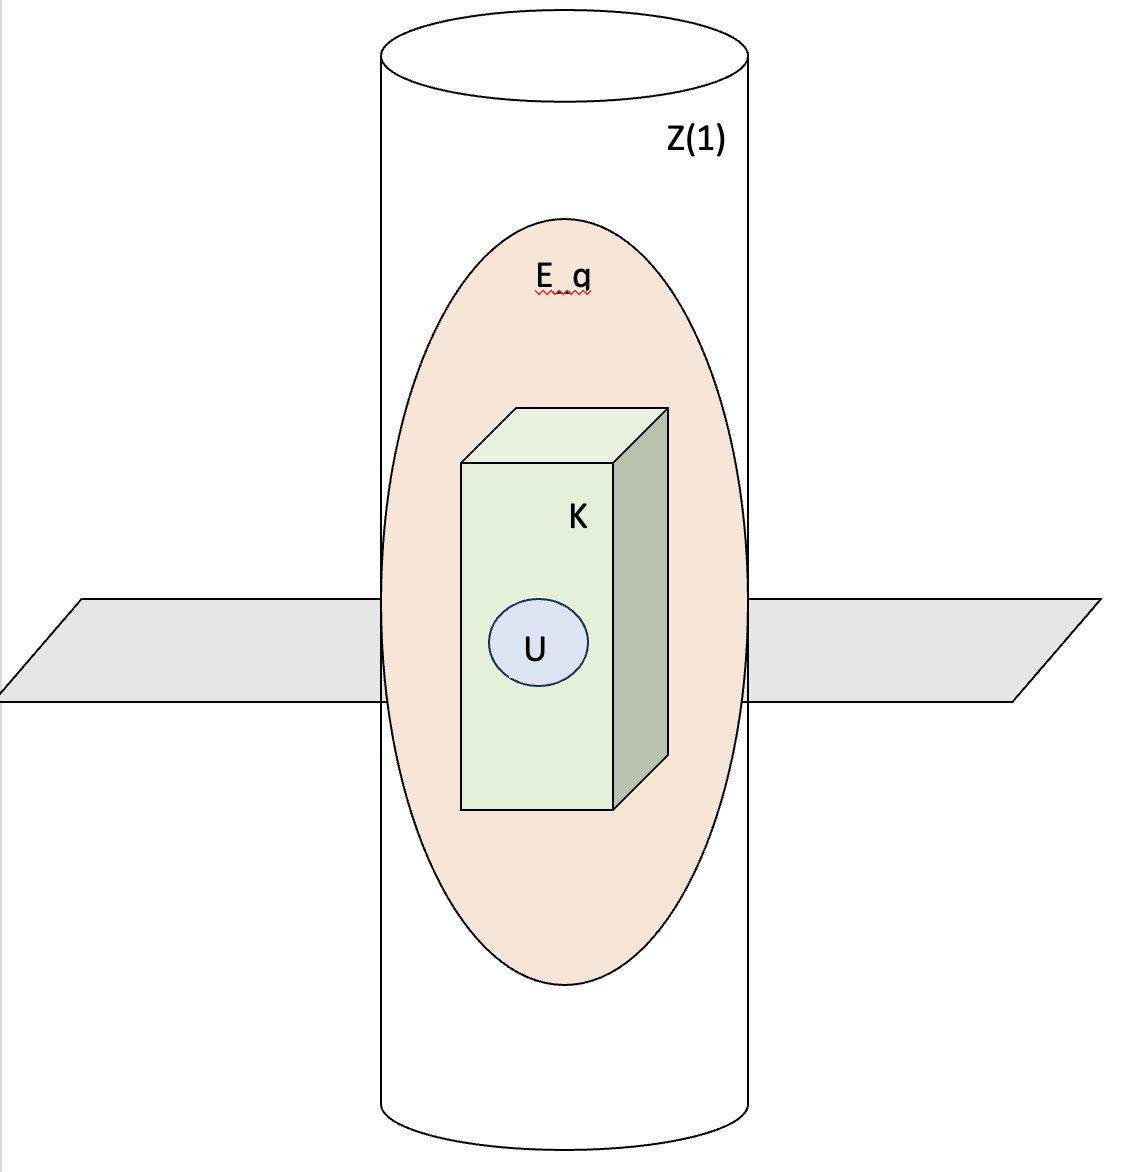
\includegraphics[width=0.5\linewidth]{images/engulfing-ellipsoid-ppt-graphic.png}
    \caption{Ellipsoid Graphic associated with large $N\in\nat^+$.}
    \label{fig:engulfing-ellipsoid}
\end{figure}
\topheader{Mollifier 2}
\begin{definition}[Mollifier 2]\label{def:mollifier-2}
    Let $f:[0,+\infty)\to\real$, smooth with
    \begin{description}
        \item[Continuity]    
        \[
        f(s) = \osc(H) \quad \forall s\leq 1
        \]
        \item[Always at least quadratic]
        \[
        f(s) \geq (\pi + \varepsilon)s\quad\forall s\in\real\footnote{this is for $\Phi\leq 0$ on $\{q>1\}$ and for the Degree Theory argument}
        \]
        \item[Almost always quadratic]
        \[
        f(s) = (\pi + \varepsilon)s\quad\forall s\text{ large.}\footnote{the difference $H(z) - Q(z)$ is $C_c^\infty(\realtn)$, and this crucial fact makes $\nabla (b\circ j)$ a compact operator on $W^{1/2}$ later}
        \]
        \item[Derivative Control]
        \[
            0 < \mathring{f}(s)\leq\pi+\varepsilon\quad\forall s>1\footnote{this is for $\Phi\leq 0$ on $\{q>1\}$}
        \]
    \end{description}
\end{definition}
\begin{definition}[Quadratic Extension of $H$]
    Let $\cl{H}:\realtn\to\real$ be defined by
    \[
        \cl{H}(z) = \begin{cases}
            H(z) & z\in E = \{q<1\} \\
            f(q(z)) & z\notin E
        \end{cases}.
    \]
\end{definition}
\begin{description}
    \item[Quadratic at Infinity] $\cl{H}(z) = Q(z) = (\pi + \varepsilon)q(z)$ for $\abs{z}\geq R$.
    \item[Vanish about origin] $\cl{H}(U) = H(U) = 0$ for some neighbourhood $U$ of $0$.
    \item[Constant about $\partial E$] There exists $0<s_0<s_1<1$ where 
    \[\cl{H}(\{s_0<q<s_1\}) = H(\{s_0<q<s_1\}) = \osc(H).\]
    That is to say, every point $z\in \{s_0<q<s_1\}$ is a critical point of $X_{\cl{H}}$.
\end{description}
\begin{wts}[Quadratic Extension is smooth]
    $\cl{H}$ is in $C^\infty(\realtn,\real)$.\footnote{see notebook page 120}
\end{wts}
\begin{proof}
    Since $f(q(z)) = \osc{H} =H(z)$ for all $q(z)\in (s_0, s_1)$, we can rewrite $\cl{H}$:
    \[
        \cl{H}(z) = \begin{cases}
            H(z) & q(z) \in(-\infty, s_1) \\ 
            f(q(z)) & q(z)\in (s_0,+\infty)
        \end{cases}
    \]
    which define $\cl{H}$ in a piecewise manner on overlapping open sets.
\end{proof}
\topheader{Construction of Mollifier 2 in \Cref{def:mollifier-2}}
\begin{description}
    \item[Standard Bump Function] Let $\phi$ be as in Mollifier 1 which normalized so that $\int\phi(x)dx = 1$.
    \item[Shrinking $\phi$ by $\delta$] Let $\phi_\delta(x) = \delta^{-1}\phi(x\delta^{-1})$, noting that $\int\phi_\delta(x)dx = \int\phi(x)dx = 1$, and $\supp{\phi_\delta} = [-\delta,+\delta]$.
    \item[Parameters] Since $(\pi + \varepsilon)<\osc(H)$, we can find $\delta>0$, where
    \[
        \osc(H) = (1+\delta)(\pi+\varepsilon)
    \]
    \item[Convolution] Let $l(x) = \max((\pi + \varepsilon)x,0)$, and 
    \[
        f_0(x) = (\phi_\delta\ast l)(x)=\int_{-\infty}^{+\infty}\phi_{\delta}(y)l(x-y)dy=\int_{-\delta}^x \phi_\delta(y)l(x-y)dy
    \]
    \item[Derivative Control] Using $D(h_1\ast h_2) = h_1\ast (D h_2)$ for suitable $h_1, h_2$, we see that $\abs{\mathring{f}_0(x)}\in[0,\pi+\varepsilon]$.
    \item[Affine Transformation] We shift $f_0(x)$ back into place by
    \[
        f(x) = f_0(x-(1+\delta)) + \osc(H)
    \]
    and this produces the plot as shown in \Cref{fig:mollifier-2-zoomed-out}.
\end{description}
\topheader{Construction of Engulfing Ellipsoid in \Cref{fig:engulfing-ellipsoid}}
\begin{description}
    \item[Quadratic Bounds on $K = \supp{X_H}$]
    \[
    c_1 = \sup_{x\in \supp{X_H}} x_1^2 + x_{n+1}^2 < 1\qqtext{and} c_2 = \sup_{x\in\supp{X_H}} \sum_{i=2}^n x_i^2 + x_{n+i}^2 < +\infty.
    \]
    \item[Choice of $N$]
    Let $N\in\nat^+$ be so large that $N^{-2}c_2<(1-c_1)$, then
    \[
        x_1^2 + x_{n+1}^2 + N^{-2}\sum_{i=2}^n x_i^2 + x_{n+i}^2 \leq c_1 + c_2N^{-2}<1.
    \]
    \item[Define $q(x)$]
    Let $q(x) = x_1^2 + x_{n+1}^2 + N^{-2}\sum_{i=2}^n x_i^2 + x_{n+i}^2$, where $q\in C^\infty(\realtn,\real)$.
    \item[Bounding $q$ on $\supp{X_H}$]
    Let $c_3 = \sup_{x\in \supp{X_H}}q(x)$, then $c_3 < 1$.
    \item[A strip about $\supp{X_H}$]
    We note that, there exists $s_0,s_1<1$ where $c_3<s_0<s_1<1$, and for all $z\in q^{-1}(s_0,s_1)$, $q(z)\in Z(1)\setminus \supp{X_H}$.
    \item[$q$ does not define $Z(1)$]
    There exists $z^*\in Z(1)$ where $q(z^*) > 1$. 
\end{description}
\begin{figure}
    \centering
    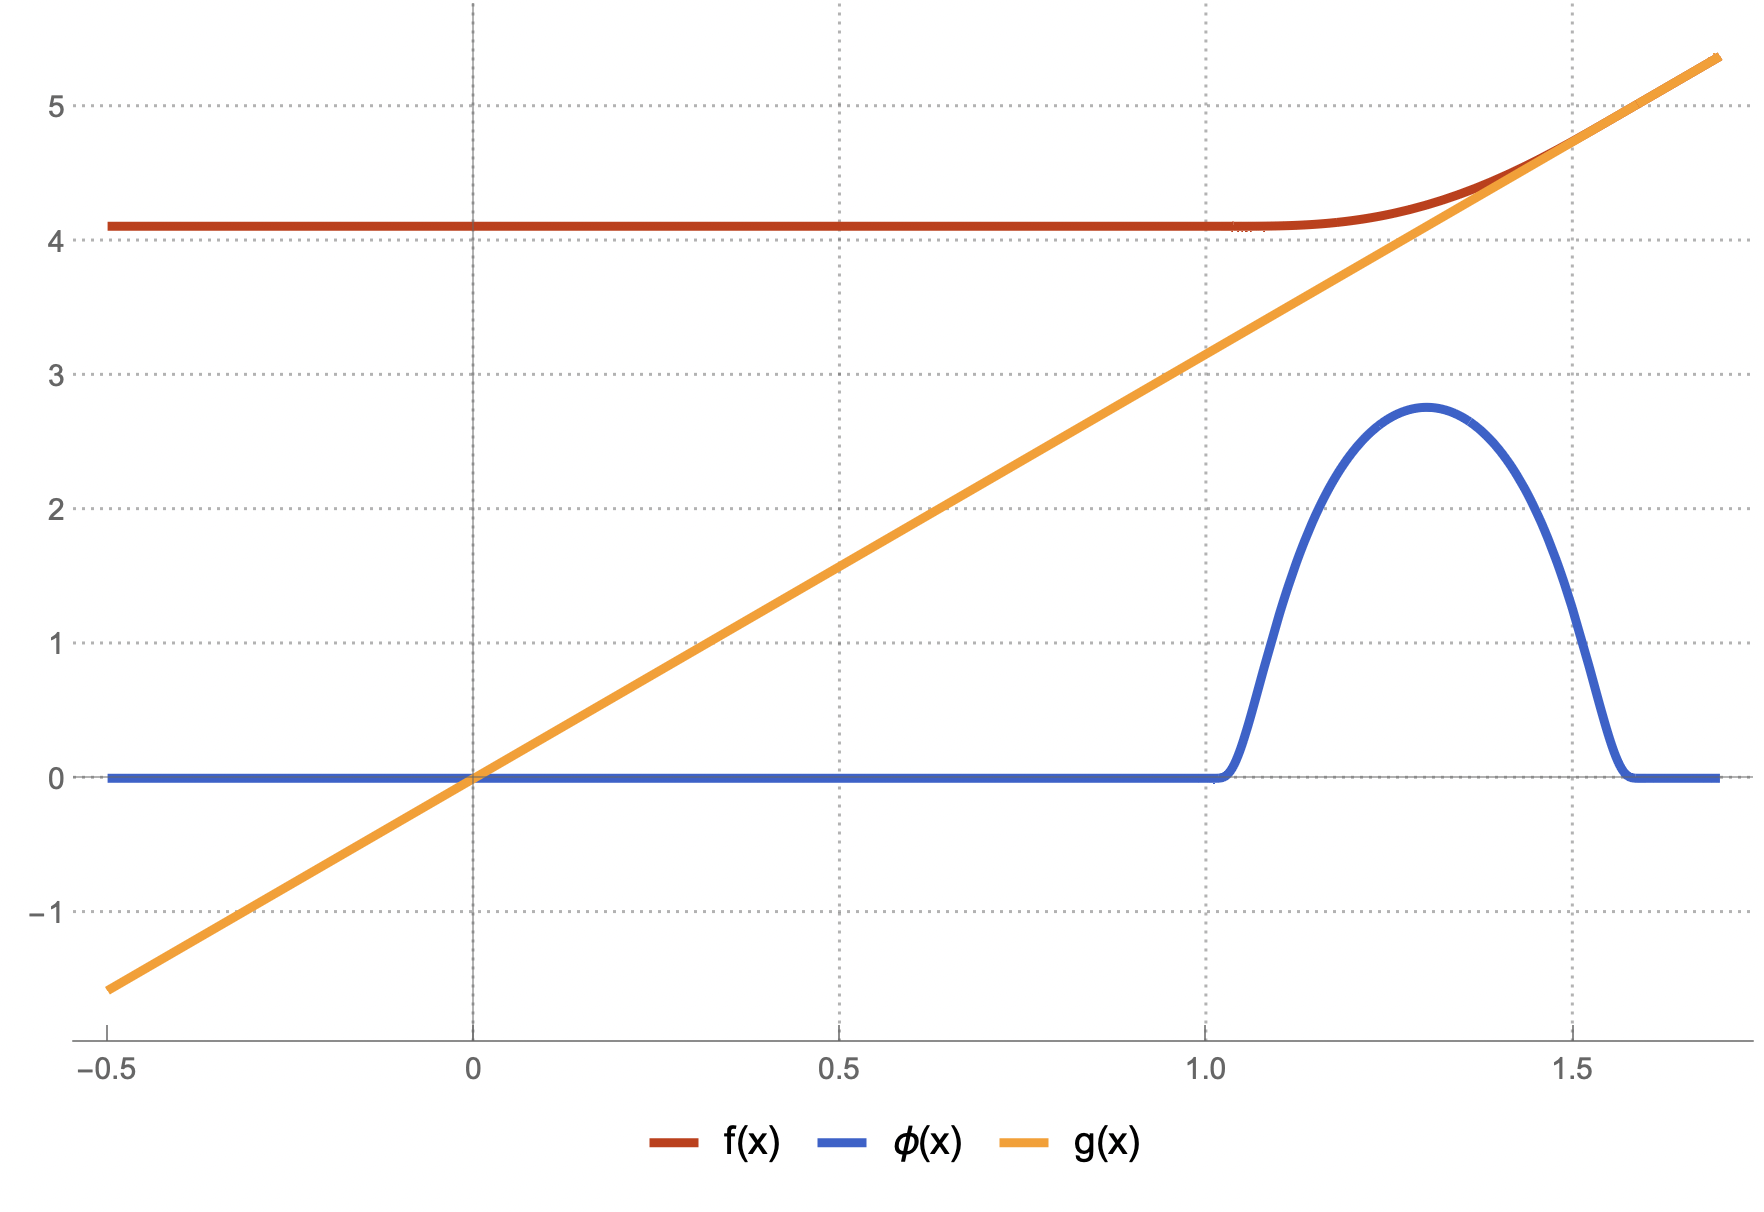
\includegraphics[width=0.8\linewidth]{images/mollifier-2-zoomedout.png}
    \caption{Mollifier 2. \texttt{Mollifier-2.nb}. $\varepsilon = 0.02$, $\delta=0.3$}
    \label{fig:mollifier-2-zoomed-out}
\end{figure}
\clearpage
\topheader{Localization of Solution}
\begin{definition}[$\Phi$ Functional]
    Let $\Phi:C^\infty(S^1,\realtn)\to\real$,
    \begin{align*}
        \Phi(x) &= 2^{-1}\int_0^1\langle \mathring{x},\ x\rangle_{\omega_0} dt- \int_0^1 H(x)dt\\[1ex]
        &=a(x) - b(x).
    \end{align*}
\end{definition}
\begin{wts}[Localization inside $E = \{q<1\}$]\label{thm:localization-theorem}
    Let $x\in C^\infty$ satisfy $\mathring{x} = X_{\cl{H}}(x)$\footnote{this is the extended system}, if 
    \[
        \Phi(x)>0,
    \] 
    then $x$ is an orbit, and $x(t)$ lies entirely within $E$\footnote{meaning $x(t)$ is a periodic orbit of our original Hamiltonian before quadratic extension}.
\end{wts}
\begin{proof}[Proof of \Cref{thm:localization-theorem}]
    We will use the contrapositive. If $x$ is constant, then $a(x) = 0$, and because $\cl{H}(z)\geq 0$ pointwise, we see that $\Phi(x)\leq 0$.\\

    Notice that if $x(t)$ intersects $\partial E$, then $x(t)$ is constant, and we can assume that $q(x(t))>1$. \\

    Because $\mathring{f}(s)>0$ for all $s>1$, we see that $q$ is conserved on $x$, as
    \[
        \{\cl{H},q\}_{\text{Poisson}} = \mathring{f}(q(z))\langle\nabla q,\ \nabla q\rangle_{\omega_0} = 0.
    \]
    Let $c = q(x)$, we can now compute $\Phi$ directly:
    \begin{align*}
    a(x) &= 2^{-1}\int_0^1 \langle\mathring{x},\ x\rangle_{\omega_0}dt = 2^{-1}\int_0^1 \langle \nabla\cl{H}(x),\ x\rangle_{\realtn}dt\\[1ex]
    &=2^{-1}\int_0^1\mathring{f}(c)\langle\nabla x,x\rangle_{\realtn}dt=\mathring{f}(c)c.
    \end{align*}
    The second last equality is due to Euler's equation:
    \[
        \langle\nabla q(x), x\rangle_{\hcal} = 2q(x),
    \]
    for every $C^1$, $2$-homogeneous function on a real Hilbert space $\hcal$. For the second term in $\Phi$, it is simply
    \[
    \int_0^1\cl{H}(x)dt = \int_0^1f(q(x)) dt = f(c).
    \]
    Finally, because $f(c)\geq (\pi + \varepsilon)c$
    \[
        \Phi(x) = \mathring{f}(c)c - f(c)\qqtext{and}\Phi(x)\leq \qty\Big((\pi + \varepsilon)c - (\pi + \varepsilon)c)\leq 0.
    \]
\end{proof}
\begin{remark}[Importance of \Cref{thm:localization-theorem}]
    If we are able to find such a $x\in C^\infty$, where $\Phi(x)>0$, this will prove that $H$ is non-admissible, as $x$ is a periodic orbit with $T = 1$.
\end{remark}
\fchapter{13: Equations (4)}
\topheader{Informal Discussion}
\begin{remark}[Relabelling]
    We relabel $H = \cl{H}$.
\end{remark}
\begin{wts}[Principle of Least Action]\label{thm:critical-points-of-phi-informal}
    If $x\in C^\infty(S^1,\realtn)$ is a critical point of $\Phi$\footnote{in the $L^2$ sense}, then 
    \[
        \mathring{x} = X_H(x).
    \]
\end{wts}
\begin{proof}[Proof of \Cref{thm:critical-points-of-phi-informal}]
We compute the $L^2$ gradient of $\Phi$.
\[
\Phi(x+\epsilon y) - \Phi(x) = \qty\Big[a(x + \varepsilon y) - a(x)] - \qty\Big[b(x + \varepsilon y) - b(x)]
\]
\begin{description}
\item[Gradient of $a$ in $L^2$]
\[
a(x+\varepsilon y) - a(x) = 2^{-1}\int_0^1\langle \mathring{x} + \varepsilon\mathring{y},\ x + \varepsilon y\rangle_{\omega_0} - \langle \mathring{x}\ x\rangle_{\omega_0} dt
\]
which is equal to (because $a$ is symmetric),
\[
    2\varepsilon a(x,y) + \varepsilon^2 a(y).
\]
We have
\[
\nabla a(x) = 2a(x,y) =\int_0^1 \langle \mathring{x},\ y\rangle_{\omega_0}dt.
\]
\item[Gradient of $b$ in $L^2$]
By the Fundamental Theorem, denoting the gradient of $H:\realtn\to\real$ by $\nabla H$,
\begin{align*}
    b(x + \varepsilon y) - b(x) &= \int_0^1 H(x + \varepsilon y) - H(x) dt \\[1ex]
    &= \int_0^1 \int _0^1\langle\nabla H(x + s\varepsilon y),\ \varepsilon y\rangle_{\realtn}ds dt\\[1ex]
    &= \iint \langle\nabla H(x),\ \varepsilon y\rangle_{\realtn}ds dt  \\
    &\quad\quad +
    \iint\langle\nabla H(x + \varepsilon y) - \nabla H(x),\ \varepsilon y\rangle_{\realtn}ds dt
\end{align*}
which we will at this point assume that $\nabla H(x)\in L^2$, and the second term is of $o(\varepsilon)$, and
\[
    \nabla b(x) = \nabla H(x) = \nabla H\circ x
\]
\item[Derivative $\Phi$ in $L^2$] 
\[
D\Phi(x)(y) = 2a(x,y) - \langle\nabla H(x),\ y\rangle_{L^2} 
\]
where we can add a factor of $J$ on both sides of the right member, because $J_{2n} = J\in SO(2n)$,
\begin{align*}
D\Phi(x)(y) &= \langle\mathring{x},\ y\rangle_{\omega_0} - \langle X_H(x),\ y\rangle_{\omega_0}\\
&= \langle\mathring{x} - X_H(x),\ y\rangle_{\omega_0} = \langle \mathring{x} - X_H(x),\ Jy\rangle_{L^2}
\end{align*}
\item[Critical Point] If $x$ is a critical point of $\Phi$, we necessarily have $\mathring{x} - X_H(x) = 0$, and 
\[
    \mathring{x} = X_H(x).
\]
\end{description}
\end{proof}
\topheader{Fourier Series}
Let $f\in C^\infty(S^1,\realtn)$, we summarize a few of the Fourier series representations we will use. 
\begin{description}
\item[Exponential Representation]
    $\hat{f}$ will be complex valued. Let $\hat{f}(i,k)$ denote the Fourier coefficient of $f$ at the $k$th frequency in the $i$th component.
    \begin{equation}
        f(x) = \hat{f}(\cdot,0)+\sum_{i=\underline{n}}\sum_{k\in\mathbb{Z}} \begin{bsmallmatrix}
            \hat{f}(i,k) & \hat{f}(i,-k) \\
            \hat{f}(n+i,k) & \hat{f}(n+i,-k)
        \end{bsmallmatrix}\begin{bsmallmatrix}
            e^{2\pi i k x}\\ 
            e^{-2\pi i k x}
        \end{bsmallmatrix}.
    \end{equation}
\item[Trigonometric Representation]
    The frequencies range over $k\geq 0$, and have real coefficients.
    \begin{equation}
        f(x) = a(0) + \sum_{i=\underline{n}}\sum_{k>0}\begin{bsmallmatrix}
            a^c(i,k) & a^s(i,k) \\
            a^c(n+i,k) & a^s(n+i,k) 
        \end{bsmallmatrix}\begin{bsmallmatrix}
            \cos(2\pi k x) \\
            \sin(2\pi k x)
        \end{bsmallmatrix}.
    \end{equation}
\item[Symplectic Basis]
    Using the symplectic exponential, $b:\mathbb{Z}\to\realtn$, $b(k) = (b(1,k)\: \ldots \: b(2n,k))$.
    \begin{equation}
        f(x) = \sum_{k\in\mathbb{Z}}e^{2\pi k J x}b(k) = b(0) + \sum_{i=\underline{n}}\sum_{k\in\mathbb{Z}} e^{2\pi k J_2 x}\begin{bsmallmatrix}
            b(i,k) \\
            b(n+i,k)
        \end{bsmallmatrix}.
    \end{equation}
    Which can be rewritten in trigonometric functions,
    \begin{equation}
        f(x) = b(0) + \sum_{i=\underline{n}}\sum_{k\in\mathbb{Z}} \qty\Big[b(i,k)\begin{bsmallmatrix}
            1 & 0 \\
            0 & -1 
        \end{bsmallmatrix} + b(n+i,k)\begin{bsmallmatrix}
            0 & 1 \\
            1 & 0 
        \end{bsmallmatrix}]\begin{bsmallmatrix}
            \cos(2\pi k x) \\ 
            \sin(2\pi k x)
        \end{bsmallmatrix}
    \end{equation}
    \item[Trigonometric to Exponential]
    \[
        \begin{bmatrix}
            \hat{f}(i,k) \\
            \hat{f}(i,-k) \\
            \hat{f}(n+i,k) \\
            \hat{f}(n+i,-k)
        \end{bmatrix} = \begin{bmatrix}
            2 & 0 & 0 & -2i \\
            2 & 0 & 0 & +2i \\
            0 & -2i & 2 & 0 \\
            0 & +2i & 2 & 0 
        \end{bmatrix}\begin{bmatrix}
            a^c(i) \\
            a^s(n+i) \\
            a^c(n+i) \\ 
            a^s(i)
        \end{bmatrix}
    \]
    \item[Symplectic to Trigonometric]
    \[
        \begin{bmatrix}
            a^c(i) \\
            a^s(n+i) \\ 
            a^c(n+i) \\ 
            a^s(i)  
        \end{bmatrix} = \begin{bmatrix}
            1 & 1 & 0 & 0 \\
            1 & -1 & 0 & 0 \\
            0 & 0 & 1 & 1 \\
            0 & 0 & -1 & 1 
        \end{bmatrix}\begin{bmatrix}
            b(i,k) \\
            b(i,-k) \\
            b(n+i,k) \\
            b(n+i,-k) 
        \end{bmatrix}
    \]
\end{description}
\begin{remark}[Convergence of Fourier Series]
    If $f\in C^\infty$, then its Fourier series converge uniformly to $f$ along with its derivatives to $\partial^\alpha f$.
\end{remark}
\topheader{Sobolev Spaces}
\begin{definition}[Sobolev Space $W^{s,2}$]
    Let $s\geq 0$ and $A_s(k) = \delta_0(k) + \sqrt{2\pi}\abs{k}^s$ for $k\in\mathbb{Z}$.
    \[
        W^{s,2} = \bigset{\phi\in\szz',\: A_s(k)\hat{\phi}(k)\in l^2}.\footnote{where $\hat{\phi}$ is the Fourier Transform of a tempered distribution.}
    \]
     
\end{definition}
\begin{remark}[Assumption of $L^2$ Sobolev Space]
    We write $W^{s} = W^{s,2}$ from now on.
\end{remark}
\subsubsection*{Equations for $W^{s}$}
\begin{description}
    \item[Inner product] $W^{s}$ is a $\real$ Hilbert space, with inner product $\langle f,\: g\rangle_{(s)} = \langle A_s\hat{f},\: A_s\hat{g}\rangle_{l^2}$,
    \[
        \langle f,\: g\rangle_{(s)} = \langle\hat{f}(0),\: \hat{g}(0)\rangle_{\realtn} + 2\pi \sum_{k\neq 0}\abs{k}^{2s}\langle\hat{f}(k),\: \hat{g}(k)\rangle_{\realtn}.
    \]
    \item[Norm] Denoted by $\norm{f}_{(s)}$, and
    \[
        \norm{f}_{(s)}^2 = \abs{\hat{f}(0)}^2 + 2\pi \sum_{k\neq 0} \abs{k}^{2s}\abs{\hat{f}(k)}^2.
    \]
\end{description}
\begin{remark}[General Sobolev Space $W^s$]
    The real definition for $W^s$\footnote{that is valid for all $s\in\real$} is defined in terms of $B_s(k) = (1+\abs{k}^2)^{s/2}$, such that 
    \[
        W^s = \bigset{\phi\in\szz',\: B_s(k)\hat{\phi}(k)\in l^2}.
    \]
    If $s\geq 0$, one can choose $c_1 = \sqrt{2\pi}$, $c_2 = \max(2^{s/2}(2\pi)^{-1/2}, 1)$ so that they induce equivalent norms
    \[
        A_s\leq c_1 B_s\leq c_2 A_s.
    \]
\end{remark}

\topheader{Sobolev Embeddings}
\begin{lemma}[Properties of Compact Operators]
    The set of compact operators $\mathcal{K}(E,F)$ is closed. Moreover, an operator $T\in L(E,F)$ is compact iff $T^*$ is compact.\footnote{Proof is the same as Theorem 6.4 of \cite{Brezis2010Functional}, see also \cite{Yosida2012} pages 282-283.}
\end{lemma}
\begin{remark}[Notation on balls on Banach Spaces]
    \[
        B_E = \{x\in E,\ \abs{x}<1\}\qqtext{and}\cl{B}_E = \{x\in E,\ \abs{x}\leq 1\}
    \]
\end{remark}
\begin{proof}
    Let $T_n\to T$ strongly, where each $T_n$ is compact. If $\varepsilon>0$ is fixed, we obtain
    \[
        \norm{T_n - T}_{L(E,F)}<\varepsilon\qqtext{and}\cl{T_n(B_E)} \subseteq\bigcup_{\text{finite}} (y_i + \varepsilon B_F).
    \]
    We claim that $\cl{T(B_E)}\subseteq \bigcup_{\text{finite}} (y_i + 3\varepsilon B_F)$. Indeed, for every $x\in B_E$,
    \[
        T_nx\in y_i + \varepsilon B_F\qqtext{and} Tx\in T_n x + \varepsilon B_F
    \]
    which implies $Tx$ is in $y_i + 3\varepsilon B_F$ as needed.\\

    Suppose $T$ is compact, if $\{v_n\}\subseteq B_{F^*}$ is any sequence, we will show that $\{T^*v_n\}\subseteq T^*(B_{F^*})$ admits a convergent subsequence. Note that
    \[
        \langle T^*(v_n),\ x\rangle = \langle v_n,\ Tx\rangle\quad\forall x\in E.
    \]
    The closed subset $\cl{T(B_E)}\subseteq F$ is a complete, compact metric space. The family
    \[
        \fourier = \{v_n\vert_{\cl{T(B_E)}}: \cl{T(B_E)}\to\real\}
    \]
    is pointwise bounded, because $\cl{T(B_E)}$ is bounded and
    \[
        \sup_{n}\abs{\langle v_n,\ y\rangle}\leq \abs{y}\sup_{n}\norm{v_n}\leq C.\footnote{because $\sup_{n}\norm{v_n}\leq 1$}
    \]
    It is also uniformly Lipschitz (which implies equicontinuity):
    \[
        \sup_{n}\abs{\langle v_n,\ y-z\rangle}\Lsim \abs{y-z}\quad\forall y-z\in \cl{T(B_E)}
    \]
    By relabelling, we can assume $v_{n}\vert_{\cl{T(B_E)}}$ is uniformly Cauchy\footnote{with respect to the uniform norm on $\cl{T(B_E)}$}. If $x\in B_E$, then $Tx\in T(B_E)$, and because $v_n$ when restricted to $T(B_E)$ converges uniformly, this is the same as $T^*v_n$ being uniformly Cauchy in $E^*$. Indeed,
    \[
        \sup_{(n,m)}\abs{\langle T^*v_n - T^*v_m, x\rangle} = \sup_{(n,m)}\sup_{x\in B_E}\abs{\langle v_n-v_m,\ Tx\rangle}\to 0,
    \]
    and $T^*v_n$ converges strongly in $E^*$. Conversely, if $T^{**}(B_{E^{**}})$ is precompact in $F^{**}$, then
    \[
        T^{**}\circ j_E(B_E)\subseteq T^{**}(B_{E^{**}})\quad\text{is precompact as well.}
    \]
    Furthermore, $j_F \circ T = T^{**}\circ j_E$, and $j_F\circ  T(B_E)$ is precompact in $F^{**}$, since $F$ is isometrically embedded, and $j_F$ has closed range --- it is a proper map\footnote{$F$ is homeomorphic to $j_F(F)$, and if $K$ is compact in $F^{**}$, $j_F^{-1}(K)$ is homeomorphic to $F\cap K$. The latter being compact in $F^{**}$.}, and $T(B_E)$ is precompact in $F$.
\end{proof}
\begin{wts}[Sobolev Embeddings are Compact]
    Let $0\leq s < t$, the inclusion map $\iota: W^t \hookrightarrow W^s$ is compact.
\end{wts}
\begin{proof}
    Approximate using partial sums, and use decay of $W^t$ Fourier Series as follows. Define
    \[
        P_N: W^{t}\to W^{s}\qqtext{where}P_N(x) = \sum_{\abs{k}\leq N} e^{2\pi kJ t}x_k.
    \]
    For simplicity, we will use the regular Sobolev factor $A_s(k) = (1+\abs{k}^2)^{s/2}$, and
    \begin{align*}
        \norm{(P_N - j)(x)}^2_{(s)} &= \norm{\sum_{\abs{k}>N} e^{2\pi kJ t}x_k}^2_{(s)}\\[2ex]
        &\Lsim \sum_{\abs{k}>N} (1+\abs{k}^2)^{s}\abs{x_k}^2 = \sum_{\abs{k}>N} A_s^2\abs{x_k}^2\\[2ex]
        &= \sum_{\abs{k}>N}\qty[A_{t}^2\abs{x_k}^2] A^2_{s-t} \leq \norm{x}^2_{(t)}\sum_{\abs{k}>N} A^2_{s-t}
    \end{align*}
    The sequence $A_{s-t}^2(k) = (1+\abs{k}^2)^{s-t}$ is in $l^1$ whenever $2(s-t)<0$.\footnote{. Indeed, $(1+\abs{k}^2)^{s-t}\Lsim_{s-t}\sum_{\abs{p}\leq s-t}\abs{k^{2p}}$
    which is bounded above (whenever $k\neq 0$) by $\abs{k}^{2(s-t)}$.} Sending $N\to\infty$ shows that $j$ is compact.
\end{proof}
\begin{corollary}[Adjoint also Compact]
    $\iota^*: W^s \hookrightarrow W^t$ is also compact.
\end{corollary}
\begin{wts}[Sobolev Regularity (\cite{Folland2013Real} Ex. 9.22)]
    Let $s> k + 1/2$, where $k$ is a non-negative integer, then $W^s$ embeds toplinearly into $C^{k}$. Moreover,
    \[
        \norm{\partial^{\alpha} x}_u\leq \norm{\fourier(\partial^{\alpha}x)}_{l^1}\Lsim \norm{x}_{(s)}\quad\forall\abs{\alpha}\leq k
    \]
\end{wts}
\begin{proof}
    Let $x\in W^s$, and considering $x$ as a distribution: denote $\hat{x}:\mathbb{Z}\to\complex^{2n}$ as its Fourier Transform, and
    \[
        \fourier(\partial^\alpha x)(k) = (2\pi i k)^{\abs{\alpha}}\hat{x}(k).
    \]
    Whose $l^1$ norm is controlled by
    \[
        \sum_{k\in\mathbb{Z}}\abs{(2\pi i k)^{\abs{\alpha}}\hat{x}(k)}\Lsim \sum \abs{(1+\abs{k}^2)^{\abs{\alpha}/2}\hat{x}(k)}.
    \]
    We borrow a factor of $s/2$, where
    \[
        \underbracket{\abs{\alpha}/2}_{l^1} = \underbracket{s/2}_{l^2} + \underbracket{(\abs{\alpha} - s)/2}_{l^2},
    \]
    and 
    \[
        \norm{(1+\abs{k}^2)^{\abs{\alpha}/2}\abs{\hat{x}(k)}^2}_{l^1}\Lsim \norm{(1+\abs{k}^2)^{s/2}\hat{x}(k)}_{l^2} \norm{(1+\abs{k}^2)^{(\abs{\alpha} - s)/2}}_{l^2}.
    \]
    Since $(1+\abs{k}^2)^{(\abs{\alpha}-s)/2}\in l^2$, this proves $\fourier(\partial^\alpha x)\in l^1$. The remaining estimate follows from the $M$ test.\\

    Suppose $p\geq 1$, and 
    \[
        g_{\alpha} = \sum_{k\in\mathbb{Z}}(2\pi i k)^{\alpha}e^{2\pi i k t}x_k\in C(S^1,\realtn).
    \]
    A simple application of the Dominated Convergence Theorem will show
    \[
        g_0(z + s) = g_0(z) + \int_0^s g_{1}(x + t)dt\quad g_1\in C(S^1,\realtn),
    \]
    and using the Fundamental Theorem proves that $x\in C^1(S^1,\realtn)$, higher order derivatives follow upon induction.
\end{proof}
\topheader{Action Extension}

We recall that 
\[
    a: C^\infty(S^1,\realtn)\to\real\qqtext{where} a(x) = 2^{-1}\int_0^1 \langle \mathring{x}(t),\ x(t)\rangle_{\omega_0}dt
\]
\begin{wts}[Extend $a$ to $W^{1/2}$]
    Because $C^\infty$ is dense in $W^{1/2}$, extend by continuity.
\end{wts}
\begin{description}
\item[Basis in $W^{1/2}$]
    Every $x\in L^2$ or $W^{1/2}$ can be expressed $x = \sum e^{2\pi k J t}x_k$ where $x_k\in\realtn$. 
    \begin{itemize}
        \item The basis $\{e^{2\pi k J t}\}_{k\in\mathbb{Z}}$ is orthogonal in $L^2$. 
        \[
            \int_0^1 \langle e^{2\pi kJ t}x_k,\ e^{2\pi m J t}y_m\rangle_{\realtn} dt = \delta(m-k)\langle x_k,\ y_k\rangle_{\realtn}.
        \]    
        \item It is also $a$-orthogonal:
        \[
            a(e^{2\pi kJ t}x_k,\  e^{2\pi mJ t}y_m) = \delta_m^k\pi k\langle x_k,\ y_m\rangle_{\realtn}.
        \]
    \end{itemize}
\item[$a$ in terms of Fourier Coefficients]
    Let $x = \sum e^{2\pi k J t}x_k$ and $y = \sum e^{2\pi k J t}y_k$, 
    \[
        a(x,y) = \sum_{k\in\mathbb{Z}}\pi k\langle x_k, y_k \rangle_{\realtn}\qqtext{and}a(x) = \sum_{k\in\mathbb{Z}}\pi k\abs{x_k}^2.
    \]
\item[$a$ is unbounded in $L^2$]
    For $x = e^{2\pi k J t}u$, where $u\in\realtn$ has length $1$, then $ \abs{a(x)} = \pi \abs{k}$ but $\norm{x}_{L^2} = 1$.
\item[Orthogonal Decomposition (1)]
    \[
    W^{1/2} = W^{1/2}_{+}\oplus W^{1/2}_{-} \oplus W^{1/2}_{0},
    \]
    spanned by $e^{2\pi kJ t}$ for $k>0$, $k<0$, and $k=0$. 
    \item[Orthogonal Decomposition (2)] Projection maps $P^{+}$, $P^-$, $P^0$. We write $x^{\pm} = P^{\pm}x$, and $x^0 = P^0 x$.
    \item[$a(x,y)$ in $W^{1/2}$] 
        \[
        a(x,y) = 2^{-1}\langle (P^+ - P^-)x,\ y\rangle_{(1/2)}
        \]
    \item[$a(x)$ in $W^{1/2}$]
        \[
        a(x) = 2^{-1}\norm{x^+}_{(1/2)}^2 - 2^{-1}\norm{x^-}^2_{(1/2)}
        \]
    \item[Gradient of $a$]
        \[\nabla a(x) = (P^+ - P^-)x = x^+ - x^-\]
\end{description}
\topheader{Inclusion Map}
\begin{description}
    \item[Definition and adjoint] $j: W^{1/2}\to L^2$. Adjoint defined by
    \[
        \langle j(x), y\rangle_{L^2} = \langle x,\ j^*(y)\rangle_{(1/2)} \forall x\in W^{1/2},\ y\in L^2.
    \]
    \item[Computation of Adjoint]
    \[
        \langle x_0,\ j^*(y)_0\rangle_{\realtn} + (2\pi)\sum_{k\neq 0}\abs{k}\langle x_k,\ j^*(y)_k\rangle_{\realtn}
        = \langle x_0,\ y_0\rangle_{\realtn} + \sum_{k\neq 0}\langle x_k,\ y_k\rangle_{\realtn}.
    \]
    \item[Fourier Coefficients]Let $y = \sum_{k\in\mathbb{Z}} \ek y_k$, 
    \[
        j^*(y) = y_0 + \sum_{k\neq 0}\ek \dfrac{y_k}{(2\pi \abs{k})}\qqtext{or} \begin{cases}
            y_0 = j^*(y)_0 \\ 
            y_k = 2\pi \abs{k}j^*(y)_k
        \end{cases}
    \]
    \item[$W^1$ control] $\norm{j^*(y)}_{(1)}\Lsim \norm{y}^2_{L^2}$
    \begin{align*}
        \norm{j^*(y)}_{(1)} &= \sum A_1^2\abs{j^*(y)_k}^2 = \abs{y_0}^2 + \sum_{k\neq 0}2\pi \abs{k}^2 \cdot \qty\Big(\dfrac{\abs{y_k}^2}{(2\pi)^2\abs{k}^2})\\
        &= \abs{y_0}^2 + (2\pi)^{-1}\sum_{k\neq 0}\abs{y_k}^2\Lsim \norm{y}_{L^2}^2.
    \end{align*}
\end{description}
\topheader{Extension of $b$}
\begin{wts}[Pointwise Properties of $H$]
    Let $z\in\realtn$, then
    \begin{description}
        \item[Pointwise Bound] 
        \[
            \abs{H(z)}\Lsim \abs{z}^2
        \]
        \item[Gradient Bound]
        \[
            \abs{\nabla H(z)}\Lsim\abs{z}
        \]
        \item[Second Derivative Bound]
        \[
            \sup_{z}\abs{D^2 H(z)} <+\infty
        \]
        \item[Gradient is Lipschitz]
        \[
            \sup_{z\in\realtn}\abs{\nabla H(z + a) - \nabla H(z)}\Lsim\abs{a}\quad\forall a\in\realtn.
        \]
    \end{description}
\end{wts}

\begin{figure}
    \centering
    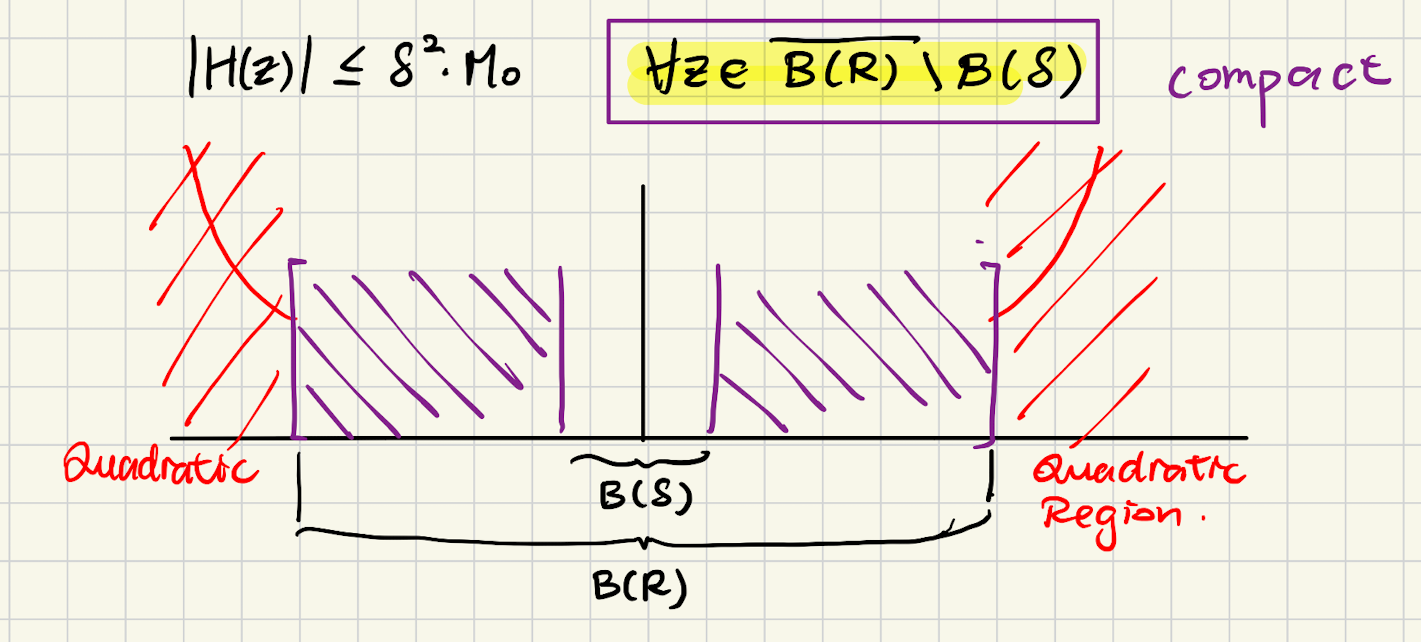
\includegraphics[width=0.75\linewidth]{images/quadratic-extension-sketch-1.png}
    \caption{Quadratic Extension Sketch 1}
    \label{fig:quadratic-extension-sketch-1}
\end{figure}
\begin{figure}
    \centering
    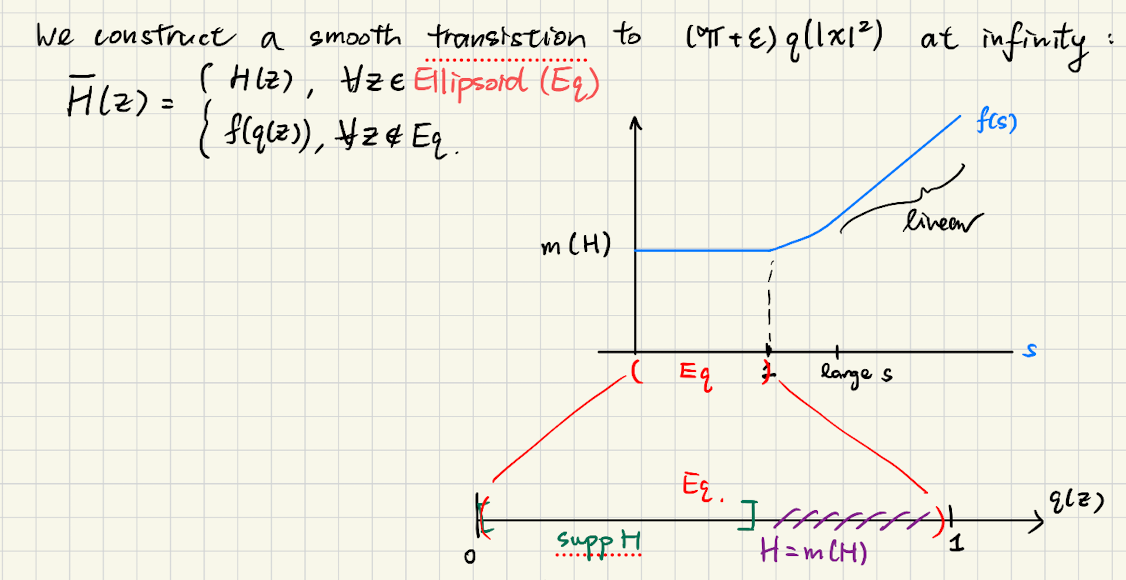
\includegraphics[width=0.75\linewidth]{images/quadratic-extension-sketch-2.png}
    \caption{Quadratic Extension Sketch 2}
    \label{fig:quadratic-extension-sketch-2}
\end{figure}
\begin{figure}
    \centering
    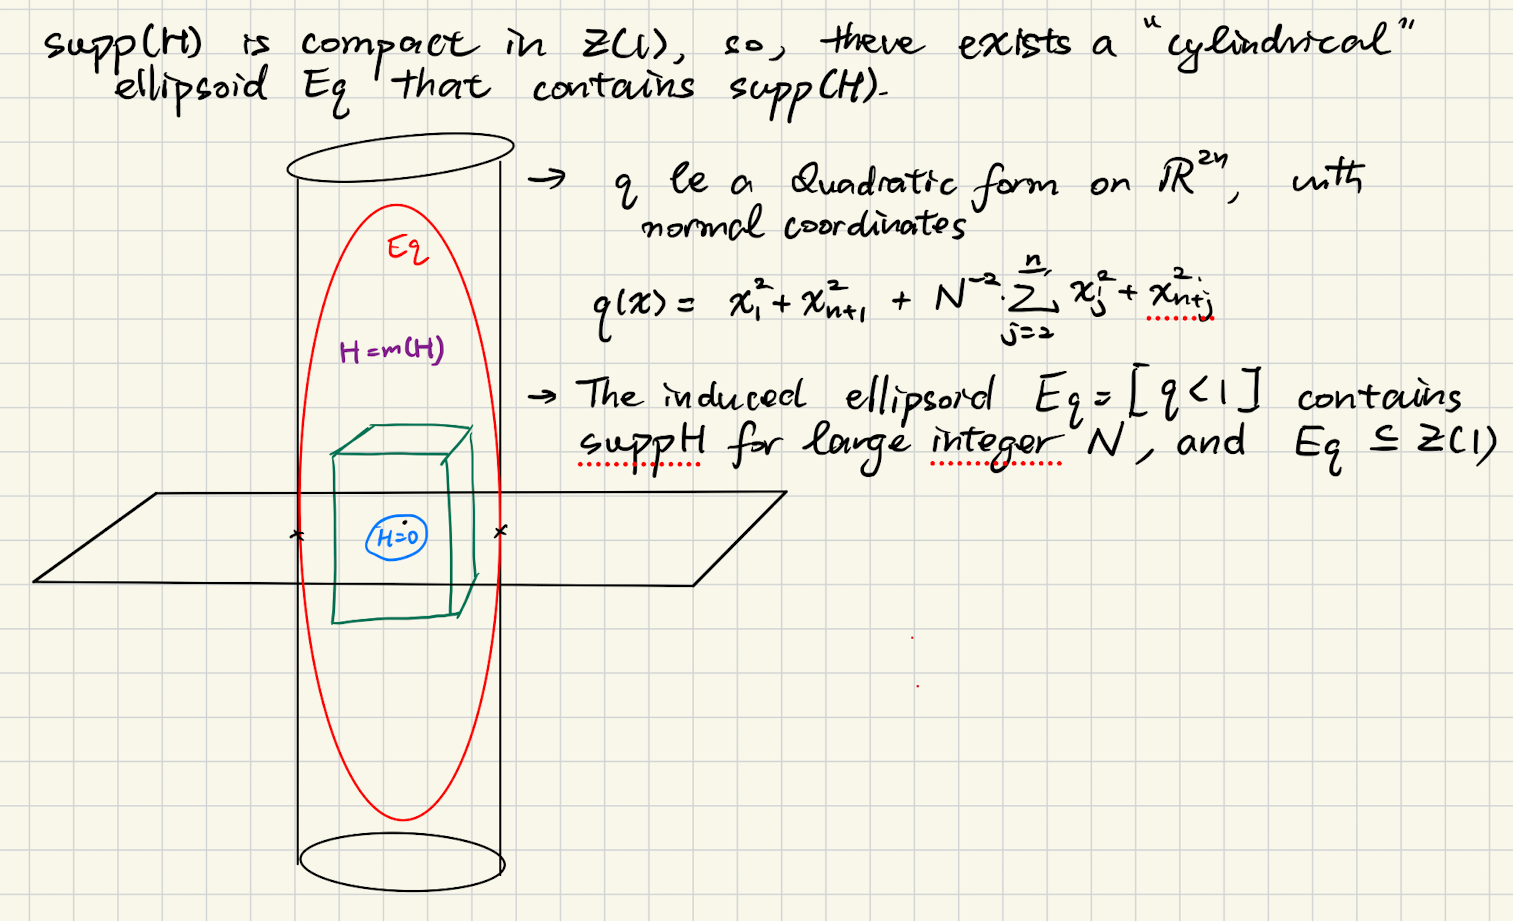
\includegraphics[width=0.75\linewidth]{images/quadratic-extension-sketch-3.png}
    \caption{Quadratic Extension Sketch 3}
    \label{fig:quadratic-extension-sketch-3}
\end{figure}
\subsubsection*{$L^2$ extension of $b$}
\begin{description}
    \item[$b$ converges in $L^2$]
    For every $x\in L^2$, the integral defining $b(x) = \int_0^1 H(x)dt$ converges absolutely,
    \[
        \abs{H(z)}\Lsim\abs{z}^2\qqtext{means}H\circ x\in L^1\quad\forall x\in L^2.
    \]
    \item[$\nabla H(x)$ is $L^2$]
    \[
        \abs{\nabla H(z)}\Lsim\abs{z}\qqtext{means}\nabla H(x) \in L^2\quad\forall x\in L^2.
    \]
    \item[$b$ is continuous]
    \[
        \abs{b(x+h) - b(x)}\Lsim \norm{DH(x)}_{L^2}\norm{h}_{L^2} + \norm{h}^2_{L^2}
    \]
    \item[$\nabla H$ is Lipschitz]
    Using the fact that $\nabla H: \realtn\to\realtn$ is pointwise Lipschitz, we see that $\nabla H:L^2\to L^2$  Lipschitz on $L^2$.
    \[
        \norm{\nabla H(x) - \nabla H(y)}^2_{L^2} \Lsim \norm{x-y}^2_{L^2},
    \]
    \item[$b$ is differentiable]
    $b\in C^1(L^2,\real)$, and 
    \[
        \nabla b(x) = \nabla H(x) \in L^2\qqtext{where}Db(x)(y) = \langle \nabla H(x),\ y\rangle_{L^2}\quad\forall x,y\in L^2.
    \]
\end{description}
\topheader{$W^{1/2}$ restriction of $b$}
Let $j:W^{1/2}\to L^2$ be the compact inclusion.
\[
    (b\circ j)(x+h) = (b\circ j)(x) + \langle \nabla H(j(x)),\ j(h)\rangle_{L^2} + o(j(h)_{(L^2)}),
\]
which gives
\[
    (b\circ j)(x+h) = (b\circ j)(x) + \langle j^*\nabla H(x),\ h\rangle_{(1/2)} + o(h_{(1/2)})\footnote{because $\norm{h}_{L^2}\Lsim \norm{h}_{(1/2)}$, and $j(x) = x$}.
\]
We can compute the $W^{1/2}$ gradient of $(b\circ j)$,
\[
    \nabla(b\circ j)(x) = j^*\nabla H(x)\quad (b\circ j)\in C^1(W^{1/2},\real).
\]
\begin{wts}[Gradient is compact]
    The mapping 
    \[
    \nabla (b\circ j):W^{1/2}\to W^{1/2}\qqtext{where}\nabla(b \circ j)(x) = j^*\nabla H(x),
    \]
    is a compact mapping. Moreover,
    \[
        \norm{\nabla (b\circ j)(x) - \nabla (b\circ j)(y)}_{(1/2)}\Lsim \norm{x-y}_{(1/2)}.
    \]
\end{wts}
\begin{proof}
Because $\nabla H: L^2\to L^2$ is Lipschitz, it maps bounded sets to bounded sets, hence $\nabla (b\circ j)$ is compact.
    \begin{align*}
        \norm{\nabla (b\circ j)(x) - \nabla (b\circ j)(y)}_{(1/2)} &= \norm{j^*(\nabla H(x) - \nabla H(y))}_{(1/2)}\\
        &\Lsim \norm{\nabla H(x) - \nabla H(y)}_{L^2} & j^* \text{ is continuous}\\
        &\Lsim \norm{x-y}_{L^2} & \text{Lipschitz on }L^2 \\
        &\Lsim \norm{x-y}_{(1/2)} & \text{Norms increase}
    \end{align*}
\end{proof}
\begin{note}[Summary]
    \begin{itemize}
    \item $j^*: L^2\to W^{1/2}$ is compact.
    \item $H(z) - Q(z)\in C_c^\infty(\realtn,\real)$.
    \item $\nabla a(x) = (P^+ - P^-)x$
    \[
        \norm{\nabla a(x) - \nabla (y)}_{(1/2)}\Lsim \norm{(P^+ - P^-)(x-y)}_{(1/2)}\Lsim\norm{x-y}_{(1/2)}
    \]
    \item $\nabla (b\circ j)(x) = j^*\nabla H(x)$ is compact.
    \[
        \norm{\nabla (b\circ j)(x) - \nabla (b\circ j)(y)}_{(1/2)}\Lsim \norm{x-y}_{(1/2)}.
    \]
    \item $\nabla \Phi(x) = (P^+ - P^-)x - j^*\nabla H(x)$
    \[
        \norm{\nabla \Phi(x) - \nabla \Phi(y)}_{(1/2)}\Lsim \norm{x-y}_{(1/2)}.
    \]
\end{itemize}
\end{note}



\topheader{Regularity of Solutions}
\begin{wts}[Critical Points of $\Phi$ are smooth]\label{thm:critical points phi smooth}
    If $x\in W^{1/2}$ satisfies $\nabla\Phi(x) = 0$, then $x\in C^\infty$, and
    \[
        \mathring{x} = X_H(x).
    \]
\end{wts}
\subsubsection*{Equations for \Cref{thm:critical points phi smooth}}
\begin{description}
    \item[Define Fourier Expansions]
   \[
    x = \sum_{k\in\mathbb{Z}} \ek x_k\qqtext{and} \nabla H(x) = \sum_{k\in\mathbb{Z}} e^{2\pi k J t}a_k.
   \]
   \item[Coefficients of $j^*\nabla H(x)$]
   \begin{align*}
    j^*\nabla H(x) &= (\nabla H(x))_0 + \sum_{k\neq 0}e^{2\pi k J t}\qty(\dfrac{(\nabla H(x))_k}{2\pi\abs{k}})\\
    &= a_0 + \sum_{k\neq 0}e^{2\pi k J t}\qty(\dfrac{a_k}{2\pi\abs{k}})
   \end{align*}
   \item[Coefficients of $(P^+ - P^-)(x)$]
   \[
    (P^+ - P^-)(x) = \sum_{k>0}e^{2\pi k J t}x_k - \sum_{k<0}e^{2\pi k J t}x_k
   \]
   \item[Compute $a_k$] Comparing Coefficients
   \[
        a_0 = 0\qqtext{and}a_k = 2\pi k x_k
   \]
   \item[Integral is $C^1$] Define
   \[
        \xi(t) = \int_0^t J\nabla H(x) ds\quad \xi\in C^1(\real,\realtn),
   \]
   (note: we cannot apply FT to $\xi$ without showing it is periodic.)
   \item[Periodicity of $\xi$]$\xi$ is periodic because 
   \[
        \int_0^1 J\nabla H(x) ds = \lim_{N\to\infty}\int_0^1\sum_{\abs{k}\leq N} J\ek a_k = 0,
   \]
   converges uniformly, DCT.\footnote{What we mean here is } 
   \item Apply Fundamental Theorem, and see that
   \[
    \mathring{\xi} = J\nabla H(x)\in L^2(S^1,\realtn),
   \]
   \item[$x$ is $C^1$] Computing $W^1$ norm by Plancherel
   \[
        \sum_{k\in\mathbb{Z}}\abs{2\pi i k}^2\abs{\xi_k}^2 = \sum_{k\neq 0}\abs{2\pi k i}^2\abs{x_k}^2 < +\infty,
   \]
   adding an adjustment term
   \[
        \sum (1+\abs{k}^2) \abs{x_k}^2 \Lsim \abs{x_0}^2 + \sum_{k\neq 0}\abs{2\pi i k}^2 \abs{x_k}^2 \Lsim \norm{(2\pi i k)\xi_k}_{l^2(\mathbb{Z})}.
   \]
   Solve for $\xi(t) = x(t) + a = \int_0^t J\nabla H(x)ds$, and $a = -x(0)$.
   \item[$x$ is $C^\infty$] by the uniqueness of integral curves:
   \[
    x(t) = x(0) + \int_0^t J\nabla H(x)ds
   \]
\end{description}

\fchapter{14: Equations (5)}
\topheader{Palais Smale Condition}
$W$ will be a Hilbert space over $\real$.
\begin{definition}[PS Condition]
    Let $f\in C^1(W,\real)$, it satisfies PS whenever every sequence $\{x_n\}\subseteq W$ with
    \[
        \sup_n \abs{f(x)}<+\infty\qqtext{and}\nabla f(x_n)\to 0,
    \]
    admits a \textbf{strongly convergent subsequence}.
\end{definition}
\begin{definition}[Minimax]
    Given a family of subsets $\mcal\subseteq \mathbb{P}(W)$, and $f: W\to\real$, the minimax is
    \[
        \text{minimax}(f,\mcal) = \inf_{E\in\mcal}\sup_{x\in E}f(x)\in\real\cup\{-\infty,+\infty\}.
    \]
\end{definition}
\begin{definition}[Positively Invariant Family]
    Let $\varphi(t,x)$ be the flow of $\mathring{x} = -\nabla f(x)$. $\mcal$ is positively invariant under $\varphi$ whenever
    \[\varphi^t(E)\in\mcal\quad\forall t\geq 0,\ \forall E\in\mcal.\]
\end{definition}
\begin{wts}[Minimax Lemma]
    Suppose $\varphi$ is a global flow, and 
    \[-\infty<\text{minimax}(f,\mcal)<+\infty.\] 
    Then there exists $x^*\in W$\footnote{not necessarily in $\mcal$. the role of $\mcal$ is just to prove the existence of $x^*$.} such that
        \[
            f(x^*) = \text{minimax}(f,\mcal)\qqtext{and}\nabla f(x^*) = 0.
        \]
\end{wts}
\subsubsection*{Equations for Minimax Lemma}
\begin{description}
    \item[Claim]
    We claim there exists $t^*>0$ such that $\sup(\varphi^{t*}(E))\leq c-\varepsilon<c$ and contradicts the assumption that $c = \text{minimax}(f,\mcal)$.
    \item If the curve $f(\varphi^{s}(x))$ intersects $(-\infty,c-\varepsilon]$ at any point in its domain, because
    \[
        f(\varphi^{t*}(x)) = f(\varphi^{s}(x)) + \int_{s}^{t}\dv{u}f(\varphi^{u}(x))du.
    \]
    The integrand follows from
    \begin{align*}
        \dv{u}f(\varphi^u(x)) &= Df(\varphi^{u}(x))\qty(\dv{u}f(\varphi^u(x)))\\[1ex]
        &= (-1)\langle \nabla f(\varphi^{u}(x)),\ \nabla f(\varphi^{u}(x))\rangle_{W} \\[1ex]
        &= (-1)\norm{\nabla f(\varphi^{u}(x))}^2_{W}
    \end{align*}
\end{description}
\topheader{Gradient Flow}

\begin{wts}[$\Phi$ satisfies PS]\label{thm:phi satisfies ps}
    Every sequence $\{x_j\}\subseteq W^{1/2}$ with
    \[
        \nabla \Phi(x_j)\to 0\quad\text{admits a convergent subsequence.}
    \]
\end{wts}
\subsubsection*{Equations for \Cref{thm:phi satisfies ps}}
\begin{description}
    \item[Periods of $X_{Q}$]
    \[
        \text{Periods} = \{\dfrac{\pi}{\pi + \varepsilon},\ \dfrac{\pi N^2}{\pi +\varepsilon}\}.
    \]
    \item[Critical Point]
    If $x$ is a critical point of $\Phi$, i.e $\nabla\Phi(x) = 0$, then
    \[
        (P^+ - P^-)(x) = j^*\nabla H(x).
    \]
    In Fourier Coefficients,
    \[
        \sum_{k>0}e^{2\pi kJt}x_k - \sum_{k<0}e^{2\pi kJt}x_k.
    \]
\end{description}
\subsubsection*{Properties of the flow}
\begin{wts}[$\Phi$ has global flow]
    The negative gradient flow of $\Phi$, 
    \[
        \mathring{x} = -\nabla \Phi(x) \quad\text{is global.}
    \]
\end{wts}
\begin{wts}[Almost Compact Flow]\label{wts:almost compact flow}
    Let $\theta(t,x):\real\times W^{1/2}\to W^{1/2}$ be the negative gradient flow of $\Phi$, then
    \[
        \theta_t(x) = e^{t}P^- + P^0 + e^{-t}P^+ + K(t,x),
    \]
    where $K:\real\times W^{1/2}\to W^{1/2}$ is compact, and 
    \[
        K(t,x) = -\int_0^t \qty\big(e^{t-s}P^- + P^0 + e^{-t + s}P^+)\nabla b(\theta(s,x))ds
    \]
\end{wts}
\begin{note}[Proper way to prove \cref{wts:almost compact flow}]
    Use Hille Yosida and $c_0$ semigroup found in Chapter 7 of \cite{Brezis2010Functional}.
\end{note}
\begin{proof}[Proof of \Cref{wts:almost compact flow}]
    We can rewrite $\mathring{x} = (-1)\nabla\Phi(x)$ in an ordinary differential equation. Recall that $\nabla\Phi(x) = (P^+ - P^-)x - \nabla (b\circ j)(x)$. If $y: I_\varepsilon\to W^{1/2}$ is an integral curve, $\dv{t}y(t) = (-1)\nabla\Phi(y(t))$ implies
    \[
    \dv{t}y(t) + (P^+ - P^-)y(t) = \nabla (b\circ j)(y(t) ).
    \]
    Notice the mapping $P^+ - P^-$ is a linear operator, and we can separate the equation into its homogenoeus and particular solutions; and we denote these by $y_h$ and $y_p$ respectively.
    \begin{description}
        \item[Commutator]
        The exponentials of $\mp tP^\pm$ are given by 
        \[
            e^{t P^-} = (e^t P^- + P^0 + P^+) \qqtext{and}e^{-t P^+} = (e^{-t} P^+ + P^0 + P^-).
        \]
        Since the commutator bracket on $L(W^{1/2})$ of $[P^+, P^-]$ is $0$, the flows induced by the two operators commute as well,
        \[
            e^{(-1)\int_0^t (P^+ - P^-)ds} = e^{t(P^- - P^+)} = e^{tP^-}e^{-tP^+}.
        \]
        Which gives us
        \[
            e^{(-1)\int_0^t P^+ - P^- ds} = (e^{-t}P^+ +P^0 + e^{t}P^-)\quad\forall t\in\real.
        \]
    \end{description}
\end{proof}
\topheader{Degree Theory}
\begin{definition}[Notation for this section]
    \begin{itemize}
        \item $\mathcal{X}(\Omega) = \{f:\cl{\Omega}\to\real,\ \text{continuous.}\}$
        \item $E,F$ = $\real$ Banach Space
        \item $L(E,F)$ = continuous linear operators.
        \item $\mathcal{K}(E,F)$ = compact operators.
    \end{itemize}
    
\end{definition}
\begin{definition}[Brouwer Degree]
The Brouwer degree takes three arguments, $d(\Omega,f,y)\in\mathbb{Z}$
\begin{itemize}
    \item $\Omega\subseteq \realn$ bounded and open, 
    \item Continuous function $f\in \mathcal{X}(\Omega)$
    \item $y\in\realn\setminus f(\partial\Omega)$
\end{itemize}
satisfies
\begin{itemize}
    \item[(d1)] $d(\id{\Omega}, \Omega, y) = 1$ for $y \in \Omega$
    \item[(d2)] $d(f, \Omega, y) = d(f, \Omega_1, y) + d(f, \Omega_2, y)$ whenever 
    \begin{itemize}[label=\textbullet]
        \item $\Omega_1, \Omega_2$ are disjoint open subsets of $\Omega$, and 
        \item $y \notin f(\bar{\Omega_1} \cup \bar{\Omega_2})$.
    \end{itemize}
    \item[(d3)] $d(h(t, \cdot), \Omega, y(t))$ is independent of $t \in J = [0, 1]$ whenever 
    \begin{itemize}[label=\textbullet]
        \item $h: J \times \bar{\Omega} \rightarrow \mathbb{R}^n$ is continuous, 
        \item $y: J \rightarrow \mathbb{R}^n$ is continuous and 
        \item $y(t) \notin h(t, \partial \Omega)$ for all $t \in J$.
    \end{itemize}
\end{itemize}
\end{definition}

\begin{definition}[Leray-Schauder Degree]
The Leray-Schauder Degree takes three arguments, $D(\Omega,F,y)\in\mathbb{Z}$
\begin{itemize}
    \item $\Omega \subseteq E$ open and bounded, 
    \item $F \in \mathcal{K}(\Omega)$ and 
    \item $y \notin (I - F)(\partial \Omega)$,
\end{itemize}
satisfies
\begin{itemize}
    \item[(D1)] $D(I, \Omega, y) = 1$ for $y \in \Omega$;
    \item[(D2)] $D(I - F, \Omega, y) = D(I - F, \Omega_1, y) + D(I - F, \Omega_2, y)$ whenever 
    \begin{itemize}
        \item $\Omega_1$ and $\Omega_2$ are disjoint open subsets of $\Omega$,
        \item $y \notin (I - F)(\bar{\Omega_1} \cup \bar{\Omega_2})$;
    \end{itemize}
    \item[(D3)] $D(I - H(t, \cdot), \Omega, y(t))$ is independent of $t \in [0, 1]$ whenever 
    \begin{itemize}
        \item $H: [0, 1] \times \bar{\Omega} \rightarrow X$ is compact, 
        \item $y: [0, 1] \rightarrow X$ is continuous and 
        \item $y(t) \notin (I - H(t, \cdot))(\partial \Omega)$ on $[0, 1]$.
    \end{itemize}
\end{itemize}
\end{definition}
\topheader{Applying Degree Theory}
\begin{definition}
    $e^+\in W^{1/2}$ with $e^+(t) = e^{2\pi Jt}e_1$ where $e_1 = (1,0,\ldots,0)\in\realtn$.
    \[
        \norm{e^+}^2_{L^2} = 1\qqtext{and} \norm{e^+}^2_{(1/2)} = 2\pi.
    \]
\end{definition}
\begin{definition}[$\Sigma_{\Tau}$ (non-positive)]
    For $\tau\geq 0$,
    \[
        \Sigma_\Tau = \bigset{x = x^- + x^0 + se^+,\ \norm{x^- + x^0}_{(1/2)}\leq \tau\ \text{and }\ 0\leq s\leq \tau}.
    \]
    Its boundary in $W_{1/2}^{-}\oplus W_{1/2}^{0}\oplus \real e^+$,
    \[
        \partial\Sigma_{\tau} = \pi^{-1}_{\leq 0}([0,\tau])\cap\pi^{-1}_{e^+}\cap\qty\Big(W_{1/2}^{-}\oplus W_{1/2}^{0}\oplus \real e^+),
    \]
    where
    \begin{itemize}
        \item $\pi_{\leq 0}:W^{1/2}\to\real$, and $\pi_{\leq 0}(x) = \norm{(P^+ - P^-)x}_{(1/2)}$,
        \item $\pi_{e^+}:W^{1/2}\to\real$, and $\pi_{e^+}(x) = (2\pi)^{-1}\langle e^+,\ x\rangle_{(1/2)}$.
    \end{itemize}
\end{definition}
\begin{wts}[$\Phi$ is non-positive on $\Sigma_{\Tau}$]\label{thm:non-positive-Sigma-Frame}
    There exists $\tau$ eventually large such that 
    \[
        \Phi\vert_{\partial\Sigma_{\Tau}}\leq 0.
    \]
\end{wts}
\subsubsection*{Equations for \Cref{thm:non-positive-Sigma-Frame} --- Part 1}
    \begin{description}
    \item[Interpolate $H$ from $Q$]
    We use the fact that 
    \[H(z) - Q(z) \in C_c^\infty(\realtn,\real)\]
        \item[Pick $\gamma = \gamma_H>0$]
        \[
            (\pi + \varepsilon)q(z) - \gamma \leq H(z)\leq (\pi + \varepsilon)q(z) + \gamma.
        \]
        \item[Bounding  $(b\circ j)(x) = \int_0^1 H(x)ds$]
        \[
            (\pi + \varepsilon)\int_0^1 q(x)ds - \gamma \leq (b\circ j)(x)\leq (\pi+\varepsilon)\int_0^1 q(x)ds + \gamma.
        \]
    \item[Estimation of $b\circ j$ using $Q$]
    \[
        \int_0^1 Q(x) dt = \sum_{k\in\mathbb{Z}}\langle x_k,\ (\pi + \varepsilon)\begin{bsmallmatrix}
            r^{-2}_{\underline{n}} & 0 \\
            0 & r^{-2}_{\underline{n}} 
        \end{bsmallmatrix}x_k\rangle_{\realtn}
    \]
    \item[Orthogonal Splitting]
    \[
        q(x^0 + x^- + x^+) = q(x^0) + q(x^-) + q(x^+)
    \]
    \[
        \int_0^1 Q(x^0 + x^- + x^+) = \int_0^1 Q(x^0) + \int_0^1 Q(x^+) + \int_0^1 Q(x^0)
    \]

    \item[Quadratic form $q$ applied to $se^+$ retrieves the first eigenvalue]
    \[
        \int_0^1 q(se^+) dt = \langle se_1,\begin{bsmallmatrix}
            r^{-2}_{\underline{n}} & 0 \\
            0 & r^{-2}_{\underline{n}} 
        \end{bsmallmatrix}se_1\rangle_{\realtn} = s^2\norm{e^+}^2_{L^2} = s^2.
    \]    
    \item[Action decomposition]
    \begin{align*}
        a(x^- + x^0 + se^+) &= 2^{-1}\langle se^+ - x^-, se^+ + x^0 + x^-\rangle_{(1/2)}\\
        &= 2^{-1}s^2\norm{e^+}^2_{(1/2)} - 2^{-1}\norm{x^-}^2_{(1/2)}.
    \end{align*}


    \item[Lower bound on norms] Pick $c = \min(2^{-1},(\pi + \varepsilon)r^{-2}_{i=\underline{n}})2^{-1}$.
    \begin{align*}
        2^{-1}\norm{x^-}^2_{(1/2)} + (\pi + \varepsilon)\langle x^0,\ [r]x^0\rangle_{\realtn} &\geq c\cdot\qty\Big(\norm{x^-}^2_{(1/2)} + \norm{x^0}^2_{(1/2)})\\
        &\geq c\cdot\qty\Big(\norm{x^- + x^0}^2_{(1/2)}),
    \end{align*}
    After shrinking $c = \min(c,\varepsilon)2^{-1}$, final inequality
    \[
        \Phi(x)\leq (-1)c\qty\Big[s^2 + \norm{x^- + x^0}^2_{(1/2)}] + (-1)\gamma
    \]
\end{description}
\begin{definition}[$\Gamma_{\alpha}$ (positive)]
    \[
        \Gamma_\alpha = \bigset{x\in W^{+}_{1/2},\ \norm{x}_{(1/2)} = \alpha}.
    \]
\end{definition}
\begin{wts}[$\Phi$ is positive on $\Gamma_{\alpha}$]
    There exists $\alpha,\beta>0$ where
    \[
        \Phi\vert_{\Gamma_{\alpha}}\geq \beta >0
    \]
\end{wts}
\topheader{Existence of Critical Point}
   
\fchapter{15: Equations (6)}
\ifSubfilesClassLoaded{% 
  \bibliography{v2-subfiles/manifolds-references}%
}{}
\end{document}